\documentclass[12pt]{article}
\parskip=\bigskipamount
\parindent=0pt
\usepackage[utf8]{inputenc}

\usepackage{geometry}[margin=1in]
\usepackage{amsmath, amssymb, amsfonts}
\usepackage{tikz}
\usetikzlibrary{shapes, backgrounds}
  \usetikzlibrary{positioning}
  \usetikzlibrary{tikzmark}
  \usetikzlibrary{arrows}
  \usetikzlibrary{calc}
  \usetikzlibrary{plotmarks}
\usepackage{booktabs}
\usepackage{natbib}
\usepackage[colorlinks=true, citecolor=blue]{hyperref}
\usepackage{listings}
\usepackage{minted}
\usepackage{changepage}
\usepackage{pgfplots}
  \pgfplotsset{compat=1.18}
\usepackage{caption}
\usepackage{subcaption}
\usepackage{float}
\usepackage{physics}
\bibliographystyle{plain}

\newcommand{\R}{\mathbb{R}}

\title{\textbf{CLASSIFICATION METHODS FOR SUPPORT VECTOR MACHINES}}
\author{\textbf{JULIA ANDRONOWITZ} \\ B.S., Mathematics}
\date{May 2023}

\begin{document}

\maketitle
\thispagestyle{empty}

\begin{adjustwidth}{0.5in}{0.5in}
\begin{abstract}
    The purpose of this thesis is to give an introduction to the concept of Support Vector Machines in Machine Learning. We will first outline the idea of classification, including the maximal margin classifier and the support vector classifier. Examples of each will be given using programming languages such as R and Python. Then, we will move onto support vector machines and the use of kernels with example data. We will implement the techniques previously described in a real data set and finish by discussing applications of SVMs and examining the documentation of the support vector machine modules in R and Python.
\end{abstract}
\end{adjustwidth}

\vfill

\begin{center}
    University of Connecticut \\ Department of Mathematics \\ Advisor: Dr. Jeremy Teitelbaum
\end{center}

\newpage

\section{INTRODUCTION}

The first discoveries regarding machine learning date back to the 1950s. Known as the "Turing Test", mathematician Alan Turing attempted to discern if a computer could fool a human into thinking it is also a human \cite{mlhistory}. In the years to follow, computer codes turned into learning programs that evolved the more times the code was run. In 1957, the first neural network was created which simulated a human brain's thought process. Ten years later, a basic pattern recognition algorithm was created called the "nearest neighbor" algorithm. Come the 1990's, accessibility to computers and advances in computers has exponentially increased. Scientists begin using a data-driven approach as large amounts of data are available, which allows computer algorithms to analyze data and learn from their results. Fast forward a few decades and we now have deep learning, survival analysis, and unsupervised learning.

Machine learning algorithms fall into one of two categories: supervised or unsupervised learning. Essentially, unsupervised learning arises when each observation does not have an associated response. This allows the machine to find certain patterns among the data and draw conclusions. Types of unsupervised learning include clustering and association. Clustering problems involve grouping the data based on the features. It is unknown how many groups are present in the data set when we begin, and so we rely on the machine to distinguish between groups. For example, we may want to group different animals based on their hunting/gathering methods and what they consume. Perhaps some animals tend to graze, others tend to scavenge, and others hunt. The algorithm would try to split the data into these three groups. In contrast, association rule learning problems focus on generalized trends between the groups. These types of trends are widely applicable to large portions of the data. For example, if one animal tends to graze on grass and other plants, the machine might suggest that another animal who grazes on grass will also eat other plants. Another common example is that people who buy one product are likely to buy another product \cite{supvunsup}.

\begin{figure}[ht]
    \centering
    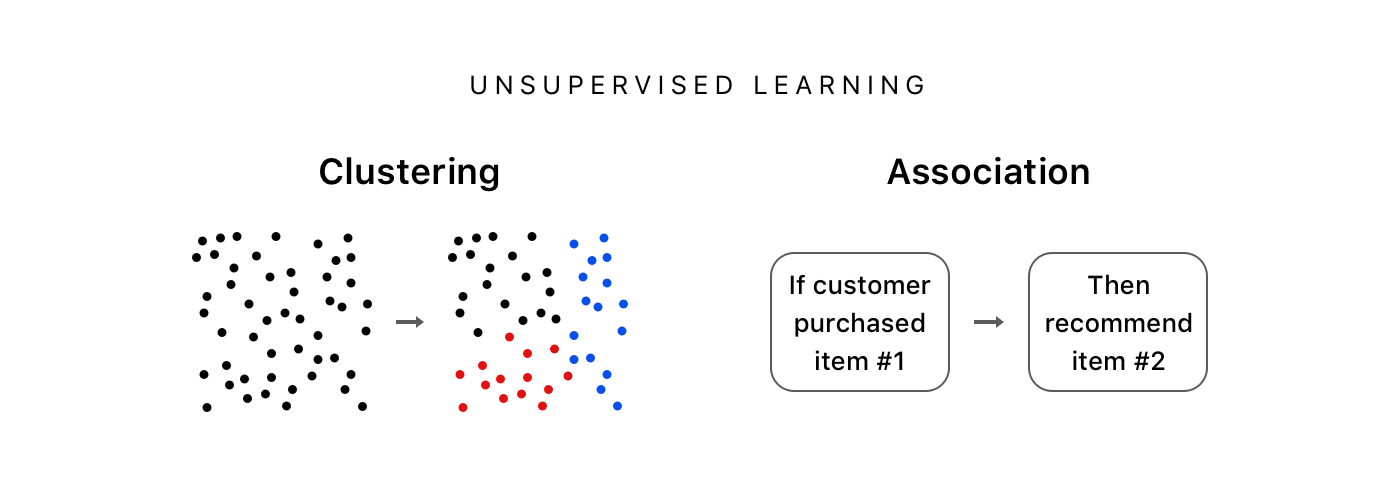
\includegraphics[height=2in]{Figures/clustering_v_association.png}
    \captionsetup[subfigure]{labelformat=empty}
    \begin{subfigure}[]{0.5\textwidth}
         \centering
         \caption{Source: Data Driven Investor}
     \end{subfigure}
    \label{fig1}
\end{figure}

In contrast, supervised learning uses data that is well-labeled to teach our model and either infer or predict. Inference problems aim for a better understanding of the relationship between the response variable and the features. On the other hand, prediction problems relate to developing a model that accurately fits the response variable to the predictors. Each observation in a data set has associated predictors and a response variable. Predictors are the input variables and can go by a variety of names such as variables, independent variables or features \cite{introstatlearning}. Predictors usually correspond to the variables $x_1,x_2,...,x_n$ where each $x_n$ is an input variable. The response variable is the dependent variable or what we are trying to measure, usually denoted as $y$. Let's take a look at some penguin data, shown in Table ~\ref{table_penguin_data}.

\begin{table}[ht]
    \centering
    \begin{tabular}{p{1.5cm}p{1.5cm}p{1.5cm}p{1.2cm}p{1.9cm}p{1.9cm}p{1.9cm}}
         Culmen Length & Culmen Depth & Flipper Length & Body Mass & Delta 15 N & Delta 13 C & Species \\
         (mm) & (mm) & (mm) & (g) & (o/oo) & (o/oo) \\
         \hline
         50.2 & 18.7 & 198 & 3775 & 9.39305 & -24.25255 & Gentoo \\
         39.5 & 17.4 & 186 & 3800 & 8.94956 & -24.69454 & Adelie \\
         44.9 & 13.8 & 212 & 4750 & 8.11238 & -26.20372 & Chinstrap \\
         52.2 & 17.1 & 228 & 5400 & 8.36701 & -25.89834 & Chinstrap \\
         50.8 & 19 & 210 & 4100 & 9.98044 & -24.68741 & Gentoo \\
         42.5 & 20.7 & 197 & 4500 & 8.67538 & -25.13993 & Adelie
    \end{tabular}
    \caption{Penguin Data}
    \label{table_penguin_data}
\end{table}

In this example, the culmen length, culmen depth, flipper length, body mass, Delta 15 N and Delta 13 C are the predictors. Based on these variables, we want the model to predict which species the penguin is. So, each body measurement is a predictor and the species is the response variable. In supervised learning, we often have training and testing groups for our data. Training and test groups are a common practice in machine learning to both classify existing data points and assess the underlying accuracy of the model on known data. Training data is data used to teach our model how to estimate the response variable. Once the model is trained, we can apply the algorithm to the testing data which the model has not previously seen. Since we already have the response variable for this set in the original data, we can compare the model's predicted $y$-values, denoted $\hat y$, with the actual $y$-values. In machine learning, it is common to see the data split into about 80\% training and 20\% testing data, but these values can be manually specified in the code \cite{trainingvtest}. Suppose we collect the data for the ten students at the end of the year. Then, we have all their test scores for the year. We take 8 students and train the model based on these observations. Then, we use the remaining two students as the test set. 

Supervised learning can be categorized into either regression or classification problems. Generally, this has to do with the fact that data is either qualitative (categorical) or quantitative (numerical). Regression typically uses a quantitative response variable. In regression, we aim to create a model that uses features to accurately predict the response variable. We may want to see how a population's access to clean drinking water impacts their average life expectancy. Linear regression can be used in this case to see whether a correlation between the two variables exist and how strong that correlation is. We can also look at how accurate the model is at predicting the response variable as well as investigate whether the relationship is linear or non-linear. On the other hand, classification is common with a quantitative response variable. In these types of problems, the data is grouped into specific categories based on the given features. The model then is able to predict the category of an unknown data point. Similarly, we can also use tools to predict the accuracy of the model and determine if the relationship is linear or non-linear.

Developed in the 1990s, support vector machines are an approach to classification problems now widely used among data scientists. In the following paper, we will discuss what a support vector machine is, how one can be implemented among a data set and practical applications of SVMs.

\section{HYPERPLANES}

We first begin by defining a hyperplane. Specifically, a hyperplane is "a flat affine subspace of dimension $p-1$" in a $p$-dimensional space \cite{introstatlearning}. In the two-dimensional space, a hyperplane looks like a straight line bisecting the data points into two distinct groups. We call this data linearly separable, as the data can be separated into two distinct groups by the hyperplane. In three dimensions, we see the formation of a plane. In higher dimensions, it can be hard to visualize the hyperplane, but the concept still applies.

Mathematically, a hyperplane in $\R^2$ is the equation $0=\beta_0+\beta_1x_1+\beta_2x_2$. Note that this is the equation of a one-degree polynomial, or a straight line. In higher dimensional spaces, a hyperplane has the form $$0=\beta_0 + \beta_1 x_1 + \beta_2 x_2 + \cdot \cdot \cdot + \beta_p x_p$$ We can generalize the equation of a hyperplane to be $$f(x)=\beta_0 + \beta \cdot x$$ where $f(x)=0$ and $\beta$ is a non-zero vector $\beta=(\beta_1,\beta_2,...,\beta_p)$ in $\R^p$ in which the dot product of $\beta$ and $x$ is computed. For any $x=(x_1,x_2)^T$ where the equation holds, we say the point is on the hyperplane. However, points that do not lie on the hyperplane will have $$0 \ne \beta_0 + \beta \cdot x$$ Moreover, the points that have $0>\beta_0 + \beta \cdot x$ will lie on one side of the hyperplane while the points $0<\beta_0 + \beta \cdot x$ will lie on the other. In this, we can see the concept of linearly separability. In a data set that is linearly separable and each observation is in one of two distinct groups, the hyperplane will bisect the data points in such a way that every point in one group is greater than zero while every point in the alternate group is less than zero.

To examine a hyperplane in two dimensions, we generate two distinct groups of data using \textit{R}.

\begin{minted}[breaklines]{R}
    n <- 200
    x1 <- matrix(rnorm(n*2, 1,0.3), ncol=2)
    x2 <- matrix(rnorm(n*2,-1,0.3), ncol=2)
    x <- rbind(x1,x2)
\end{minted}

We first set $n=200$. This will be the length of our data set. Then, we use the function \textbf{rnorm} to generate a set of data points from the normal distribution with mean 1 and standard deviation 0.3. The matrix function transforms the 400 randomly generated points into a [200 x 2] matrix. The same is done for a second group, instead with mean $-1$ and standard deviation 0.3. The \textbf{rbind} function combines these two groups into one vector, namely $x$.

\begin{minted}[breaklines]{R}
    plot(x,xlab="",ylab="")
    abline(h=0,v=0,col="gray",lty="dotted")
    abline(a=0,b=-1,col="black",lty="dashed")
\end{minted}

Now, we plot the function. The \textbf{abline} functions add lines at $x=0$ and $y=0$ as well as add one such separating hyperplane. Figure ~\ref{fig_mmc_separating_hyperplane} shows the output.

\begin{figure}[ht]
\begin{center}
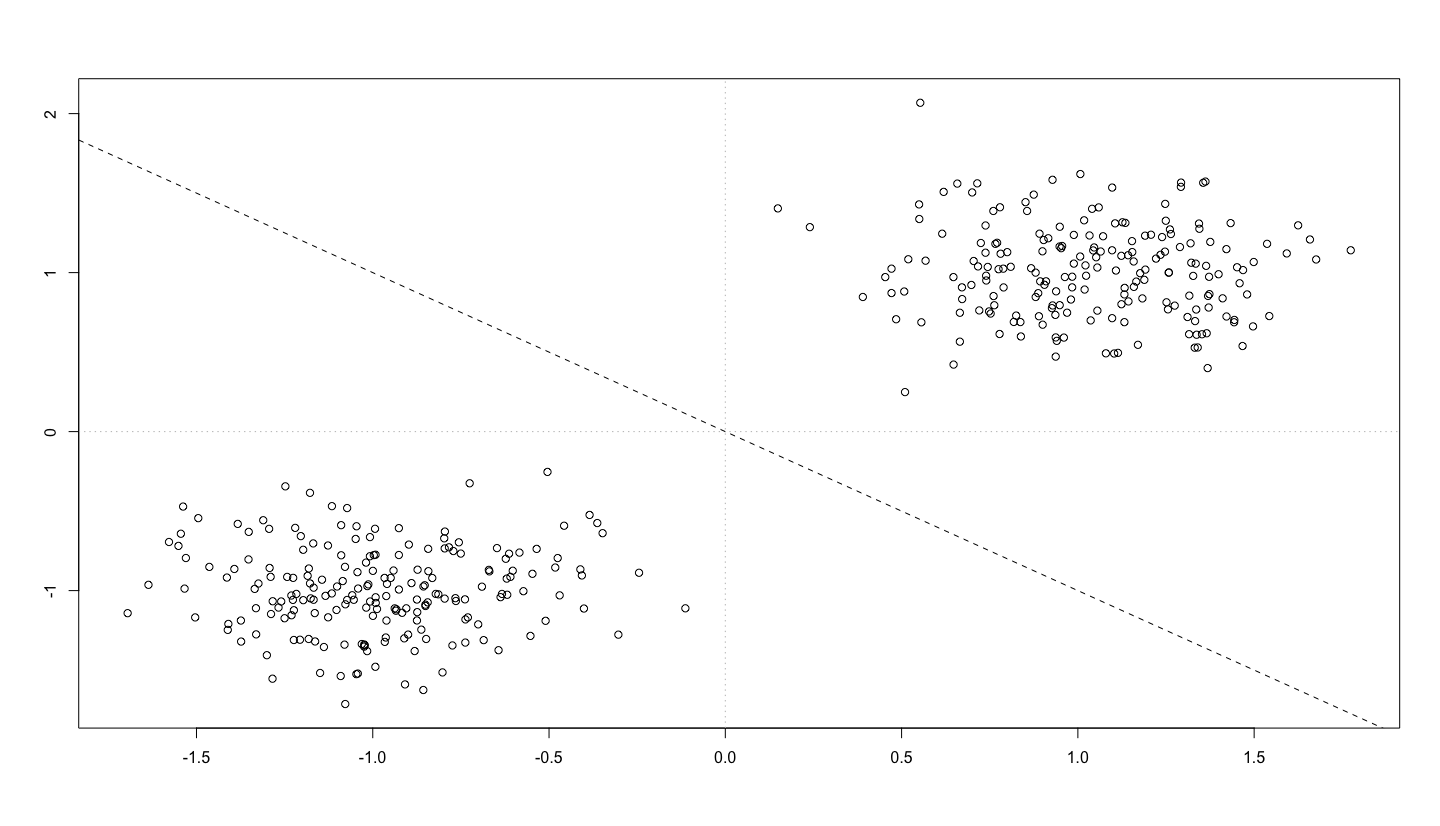
\includegraphics[width=5.5in]{Figures/mmc/mmc_separating_hyperplane.png}
\caption{Randomly Generated Clustered Data \\ with Separating Hyperplane in $\R^2$}
\label{fig_mmc_separating_hyperplane}
\end{center}
\end{figure}

We see that there is a clear separation between the data points and a hyperplane that bisects the data. The equation of the hyperplane in this example is defined by $y=-x$. In the form $f(x)=\beta_0 + \beta \cdot x$, we have $f(x)=0$, $\beta_0=0$, and $\beta=(1,1)$ to give $0=0+x_1+x_2$ or $x_1=-x_2$.

Notice that we can rotate the line slightly in either direction and still have separating hyperplane. So long as the line does not pass through the points that the gray line intersects, there exist infinitely many such separating hyperplanes. An example is shown in red in Figure ~\ref{fig_mmc_multiple_hyperplanes}.

\begin{figure}[ht]
\begin{center}
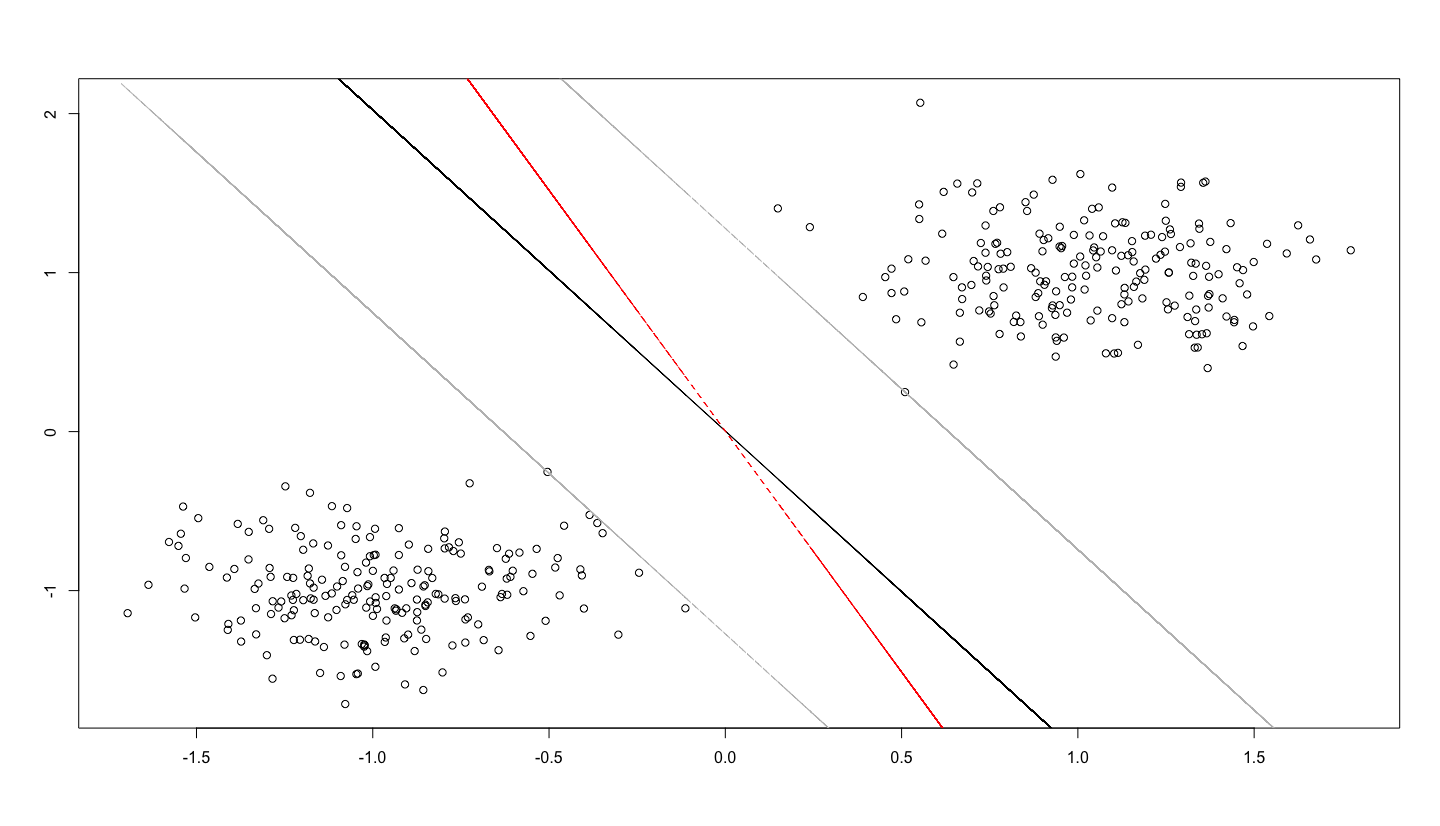
\includegraphics[width=5.5in]{Figures/mmc/mmc_multiple_hyperplanes.png}
\caption{Randomly Generated Clustered Data with Multiple \\ Hyperplanes in $R^2$}
\label{fig_mmc_multiple_hyperplanes}
\end{center}
\end{figure}

Similarly, in a three-dimensional space the hyperplane partitions the data. A plane separates the set into two distinct groups. An example can be generated with Python. 

\begin{minted}[breaklines]{R}
    data1a = np.random.normal(-1,0.3,size=(10,1))
    data1b = np.random.normal(-0.5,0.3,size=(10,1))
    data1c = np.random.normal(0,0.1,size=(10,1))

    data2a = np.random.normal(1,0.3,size=(10,1))
    data2b = np.random.normal(0.5,0.3,size=(10,1))
    data2c = np.random.normal(0,0.1,size=(10,1))
\end{minted}

These functions set up our two data sets. The $a, b, c$ values correspond to the $x,y,z$ coordinates for each set. A randomly generated sample from the normal distribution is used. We then create the graph by setting up the axes and writing the equation for the hyperplane that will bisect the data before plotting the points.

\begin{minted}[breaklines]{python}
    x = np.linspace(-1, 1, 10)
    y = np.linspace(-1, 1, 10)

    x, y = np.meshgrid(x, y)
    eq = 1 * x + 0.15 * y

    fig = plt.figure()
    ax = fig.gca(projection='3d')
    ax.plot_surface(x, y, eq, color='green',alpha=0.3)

    ax.scatter(data1a,data1b,data1c, color='black')
    ax.scatter(data2a,data2b,data2c, color='black')

    plt.show()
\end{minted}

The output is shown in Figure ~\ref{fig_randomly_generated_R3}.

\begin{figure}[ht]
    \centering
    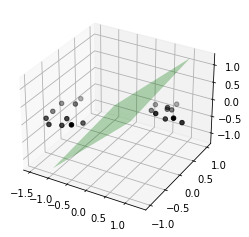
\includegraphics{Figures/randomly_generated_R3.png}
    \caption{Randomly Generated Clustered Data \\ with Separating Hyperplane in $\R^3$}
    \label{fig_randomly_generated_R3}
\end{figure}

In this example, we see one set of points is to the left of the hyperplane while the other lies on the right. The equation of the hyperplane is $z = x + 0.15y$. In the form $f(x)=\beta_0 + \beta \cdot x$, we have $f(x)=0$, $\beta_0=0$, and $\beta=(1,0.15,-1)$ to give $0=0+x_1+0.15x_2-x_3$ or $x_3=x_1+0.15x_2$. Like in the two-dimensional case, there is an infinite number of separating hyperplanes in three dimensions. By slightly rotating the plane shown in Figure ~\ref{fig_randomly_generated_R3} in either direction, we can visualize the concept of numerous other planes that would bisect the same data set.

\section{MAXIMAL MARGIN CLASSIFIER}

The use of hyperplanes to distinguish between two classes is central to the maximal margin classifier. Also called the optimal margin classifier, this method aims to find the separating hyperplane that maximizes the distance between the two sets of points. That is, if the plane were to rotate slightly in either direction, it would be closer to the set of data points. Our depiction of the maximal margin classifier draws upon those presented in \cite{introstatlearning} and \cite{teitelbaum2021svmnotes}.

In the above example, we can classify each set of points to determine what side of the hyperplane they lie on. So, if $y_i=1$ then $0>\beta_0 + \beta \cdot x$ and if $y_i=-1$ then $0<\beta_0 + \beta \cdot x$. Each $y_i$ becomes the class label for that observation. Class labels are the identifiers for the data points and distinguish which class the observation belongs to. Introducing the following starred lines to our code produces colors in the graph according to the respective group:

\begin{minted}[breaklines]{R}
    # setting initial number of observations in each set
    n <- 200
    
    # calculating x-variable using two randomly generated sets with overlap
    set.seed(100)
    
    mmcdatax1 <- matrix(rnorm(n*2, 1,0.3), ncol=2)
    mmcdatax2 <- matrix(rnorm(n*2,-1,0.3), ncol=2)
    mmcdatax <- rbind(mmcdatax1,mmcdatax2)
    
    # assigning labels to both classes
    mmcdatay <- c(rep(-1,n), rep(1,n))
    
    # plotting the data
    plot(mmcdatax, col=(3-mmcdatay),xlab="",ylab="",pch=16)
    
    # adding line to visualize a hyperplane
    abline(h=0,v=0,col="gray",lty="dotted")
    abline(a=0,b=-1,col="black",lty="dashed")    
\end{minted}

We assign a vector of 200 negative ones followed by 200 positive ones to the variable $y$. Combined with the adjusted plot function containing the color option $(3-y)$, the first 200 points are plotted blue and the last 200 points are plotted red. This gives out two groups shown in Figure ~\ref{fig_mmc_hyperplane_w_labels}.
\begin{figure}
    \centering
    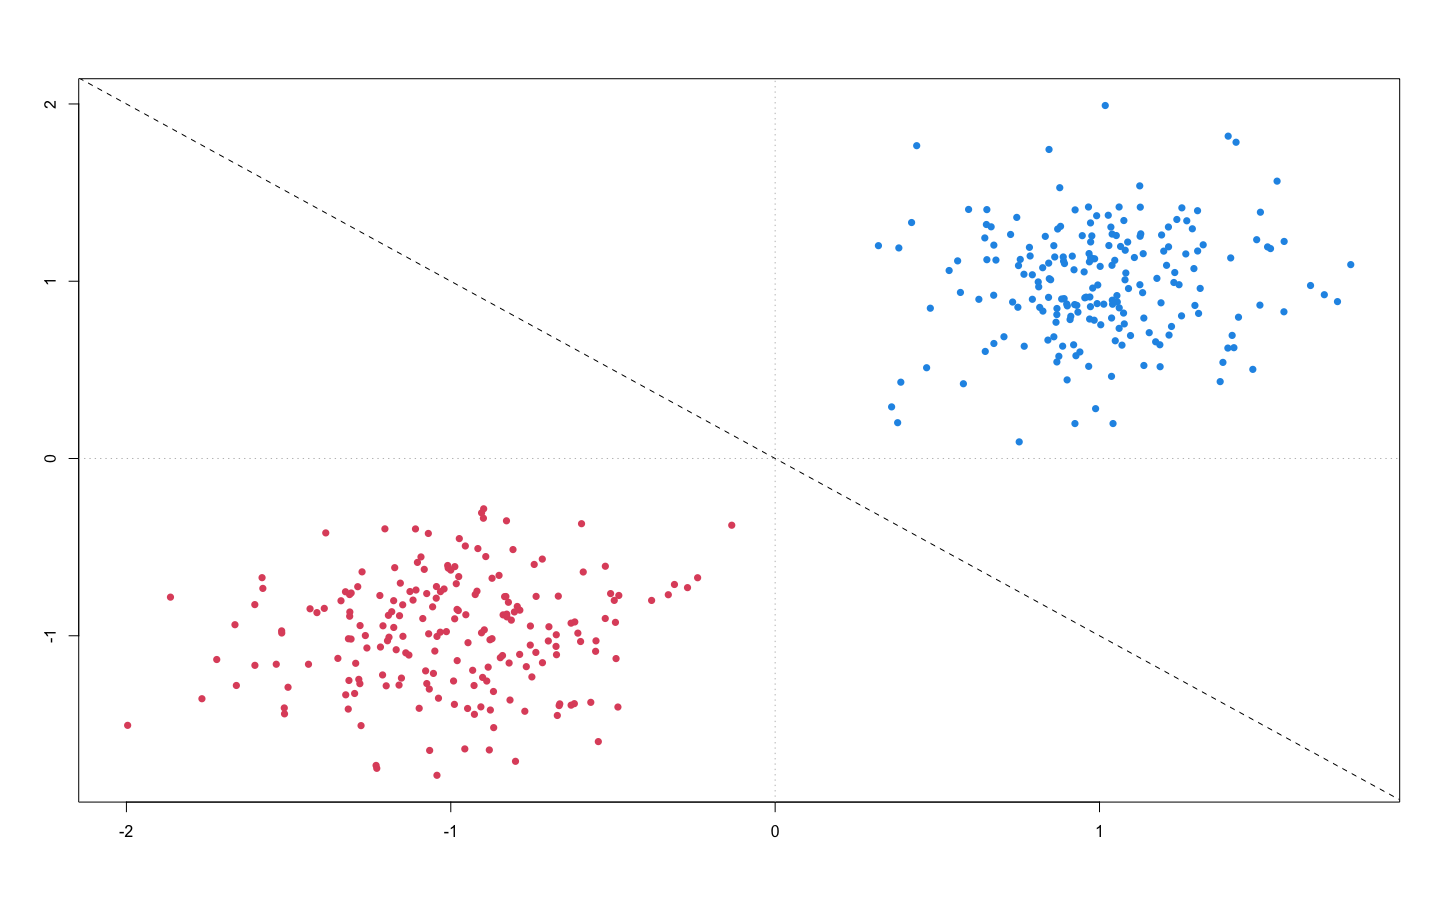
\includegraphics[width=5.5in]{Figures/mmc/mmc_hyperplane_w_labels.png}
    \caption{Randomly Generated Data with Associated Class Label Coloring}
    \label{fig_mmc_hyperplane_w_labels}
\end{figure}
We need to find the closest blue and red points such that shifting the hyperplane in any such way results in a smaller margin for either group. These points are known as the support vectors, as they are the only points that end up formulating the hyperplane. At this point, we know that points with $0>\beta_0 + \beta \cdot x$ will lie on one side of the hyperplane and have a class label $y_i$ of 1, while the points $0<\beta_0 + \beta \cdot x$ lie on the other and have a class label $y_i=-1$. Combining these two constraints, we can produce one inequality that correctly classifies each point
$$y_i(\beta_0+\beta_1x_{i1}+...+\beta_px_{ip})>0$$
\begin{figure}[ht]
    \centering
\begin{tikzpicture}[scale=1.5]
    \begin{axis}[
        xticklabel=\empty,
        yticklabel=\empty
    ]
        \addplot[<->,domain=-10:10,samples=100]({x},{-x});
    \end{axis}
    \draw (1,5) node[right] {$0=\beta_0+\beta_1x_1+\beta_2x_2$};
    \draw (5.7, 4.055) node[left] {$\theta$};
    \draw (5.1,3.255) node[right] {$\vec{n}$};
    \draw (4,4) node[above] {$\vec{v}$};
    \draw (2.05,3.25) node[above] {($b_1,b_2$)};
    \draw (5.9,4.155) node[right] {($a_1,a_2$)};
    
    \draw[fill] (4, 2.355) circle [radius = .05 cm];
    \draw[fill=blue] (6,4.355) circle [radius = .05 cm];
    \draw[fill=blue] (6.4, 5) circle [radius = .05 cm];
    \draw[fill=blue] (6, 5.3) circle [radius = .05 cm];
    \draw[fill=blue] (5.6, 5.1) circle [radius = .05 cm];
    \draw[fill=blue] (5.85, 4.8) circle [radius = .05 cm];
    
    \draw[->] (4, 2.355) edge (6,4.355);
    \draw[->] (4, 2.355) edge (5,3.355);
    \draw[->] (6,4.355) edge (2.6,3.5);
    \draw (4.2, 2.555) edge (4, 2.755);
    \draw (4,2.755) edge (3.8,2.555);
\end{tikzpicture}
    \caption{Diagram of Hyperplane and Support Vector}
    \label{supportvectors}
\end{figure}

Suppose we look at a few points with a separating hyperplane of $0=f(x_1,x_2)=\beta_0+\beta_1x_1+\beta_2x_2$, pictured in Figure ~\ref{supportvectors}. We assume the point $(a_1,a_2)$ in the set of the positive class labels is the closest point to the set of points with a negative class label. Then, to compute the perpendicular distance $d$ from the point $(a_1,a_2)$ to $f(x_1,x_2)=0$, we first find a normal vector to $f$. Through calculus, the gradient of the hyperplane calculated by $(dx_1,dx_2)$ gives the normal vector $\vec{n}=\expval{\beta_1, \beta_2}$ to $f$. Let $(b_1,b_2)$ be any point on the hyperplane. Then $\vec{v}=(a_1-b_1,a_2-b_2)$. The distance $d$ equals $||\vec{v}|| \cos{\theta}$ through trigonometry. Then we have
\begin{align*}
    \vec{v} \cdot \vec{n}&=||\vec{v}|| ||\vec{n}|| \cos{\theta} \\
    \vec{v} \cdot \vec{n}&= d \cdot ||\vec{n}|| \\
    d &= \frac{\vec{v} \cdot \vec{n}}{||\vec{n}||} \\
    &= \frac{(a_1-b_1,a_2-b_2) \cdot \expval{\beta_1,\beta_2}}{\sqrt{\beta_1^2+\beta_2^2}} \\
    &=\frac{\beta_1a_1-\beta_1b_1+\beta_2a_2-\beta_2b_2}{\sqrt{\beta_1^2+\beta_2^2}} \\
    &= \frac{\beta_1a_1+\beta_2a_2-(\beta_1b_1+\beta_2b_2)}{\sqrt{\beta_1^2+\beta_2^2}}
\end{align*}
Since $(b_1,b_2)$ lies on the hyperplane, we have $\beta_0+\beta_1b_1+\beta_2b_2=0$ and $\beta_1b_1+\beta_2b_2=-\beta_0$. Thus,
\begin{align*}
    d&= \frac{\beta_1a_1+\beta_2a_2-(\beta_1b_1+\beta_2b_2)}{\sqrt{\beta_1^2+\beta_2^2}} \\
    &= \frac{\beta_1a_1+\beta_2a_2-(-\beta_0)}{\sqrt{\beta_1^2+\beta_2^2}} \\
    &= \frac{\beta_1a_1+\beta_2a_2+\beta_0}{\sqrt{\beta_1^2+\beta_2^2}}
\end{align*}

Note that the numerator is exactly the equation $f$. In fact, there exist infinitely many such functions, as we could simply multiply $f$ by a constant. Suppose we have the equivalent hyperplane $ 0=C\beta_1a_1+C\beta_2a_2+C\beta_0$ for any $C \in \mathbb{R}$. Then,
\begin{align*}
    d&= \frac{C\beta_1a_1+C\beta_2a_2+C\beta_0}{\sqrt{(C\beta_1)^2+(C\beta_2)^2}} \\
    &=\frac{C(\beta_1a_1+\beta_2a_2+\beta_0)}{\sqrt{C^2(\beta_1^2+\beta_2^2)}} \\
    &=\frac{C(\beta_1a_1+\beta_2a_2+\beta_0)}{C\sqrt{\beta_1^2+\beta_2^2}} \\
    &=\frac{\beta_1a_1+\beta_2a_2+\beta_0}{\sqrt{\beta_1^2+\beta_2^2}} \\
\end{align*}
Notice that we are left with the same distance $d$, even with a different equation for the hyperplane. By imposing the condition $\beta_1^2+\beta_2^2=1$, we restrict the above to just one possible hyperplane. So, we are left with $$d=\frac{f(a_1,a_2)}{\sqrt{\beta_1^2+\beta_2^2}}$$ We aim to find the greatest distance, or margin, by maximizing the coefficients to the function $f$ of the closest point(s) to the hyperplane. Thus, we have the basic idea for the maximal margin classifier. We seek to maximize the margin $M$ to find the best separating hyperplane given by

$$y_i(\beta_0+\beta_1x_{i1}+...+\beta_px_{ip}) \ge M$$

provided that

\begin{equation}\label{sumofsquares}
\sum_{j=1}^{p} \beta^2_j=1
\end{equation}

Though the maximal margin classifier is not a support vector machine quite yet, we may use the SVM module in the "e1071" library in $R$ to determine the equation of the line.

\begin{minted}[breaklines]{R}
    # creating data frame 
    mmcdata <- data.frame (x = mmcdatax, y = factor(mmcdatay))
    
    # splitting into training and test data
    library(caTools)
    set.seed(100)
    
    # using 80% of the data in the training set and the other 20% in the test set
    sample <- sample.split(mmcdata$x.1, SplitRatio = 0.8)
    train  <- subset(mmcdata, sample == TRUE)
    test   <- subset(mmcdata, sample == FALSE)
    
    # computing svm function
    svmfit <- svm (y~., data = train , kernel="linear", cost = 1000, scale = FALSE)
    
    # plotting svm function graph
    plot(svmfit,train)
\end{minted}

Once downloading the package, we assign the $x$ and $y$ variables to one dataframe. We convert the $y$ variable into a factor since class label is a binary value. In the \textbf{svm} function, the dataframe we just defined is the basis of the calculations. Note that we split the dataset into a training and a test set using the method outlined in \cite{r_train_test_split}. This allows us to train the model on 80\% of the data and use the remaining 20\% of the data as a method of validation. This is done with the "caTools" library. When computing the support vector machine, we assign the kernel as linear with a cost of 1000, though other options exist for non-separable data and non-linear decision boundaries (which we will get to in later pages). We plot the function and see the output in Figure ~\ref{fig_mmc_module_output}.

\begin{figure}
    \centering
    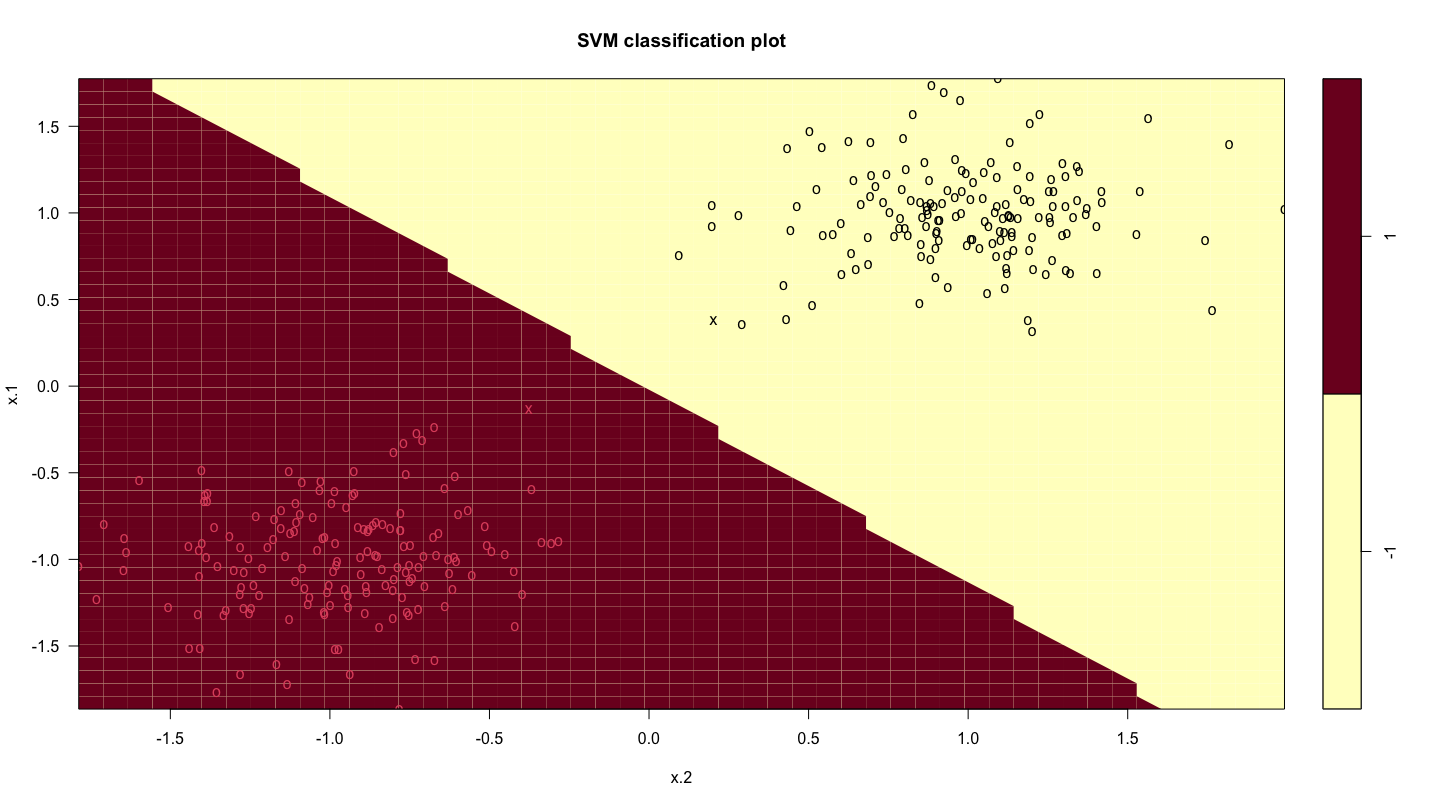
\includegraphics[width=5.5in]{Figures/mmc/mmc_module_output.png}
    \caption{Maximal Margin SVM Module Output in $R$}
    \label{fig_mmc_module_output}
\end{figure}
As we see, the separating hyperplane is illustrated clearly albeit not pictured exactly linear. Details of the \textbf{svm} function can be found using the following:
\begin{minted}[breaklines]{R}
    summary(svmfit)
    svmfit$index
    svmfit$rho
    svmfit$coefs
\end{minted}

\begin{figure}[ht]
    \centering
    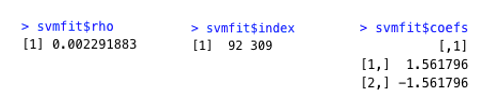
\includegraphics[width=5in]{Figures/mmc/mmc_selected_output.png}
    \caption{Selected Output of SVM Function}
    \label{fig_mmc_selected_output}
\end{figure}

The \textbf{str} function tells us that \textbf{svmfit} is a list of 30 variables, some of which we defined in the function and others that were calculated. Particularly of interest are the \textbf{index}, \textbf{rho}, and \textbf{coefs} variables, which give the output in Figure ~\ref{fig_mmc_selected_output}. The \textbf{rho} variable is the intercept of the separating hyperplane, and the \textbf{coefs} variable is an array of the coefficients of the supporting vectors. The \textbf{index} variable tells us the indices of the observations that the classifier depends on, or the support vectors. In this case, it is data points 66 and 285. If we were to rotate the hyperplane in any direction, the margin from these two points to the black line would inevitably become smaller. Visually, we can see these two points as those that the supporting hyperplanes pass through in Figure ~\ref{fig_mmc_graph}.

\begin{figure}[H]
    \centering
    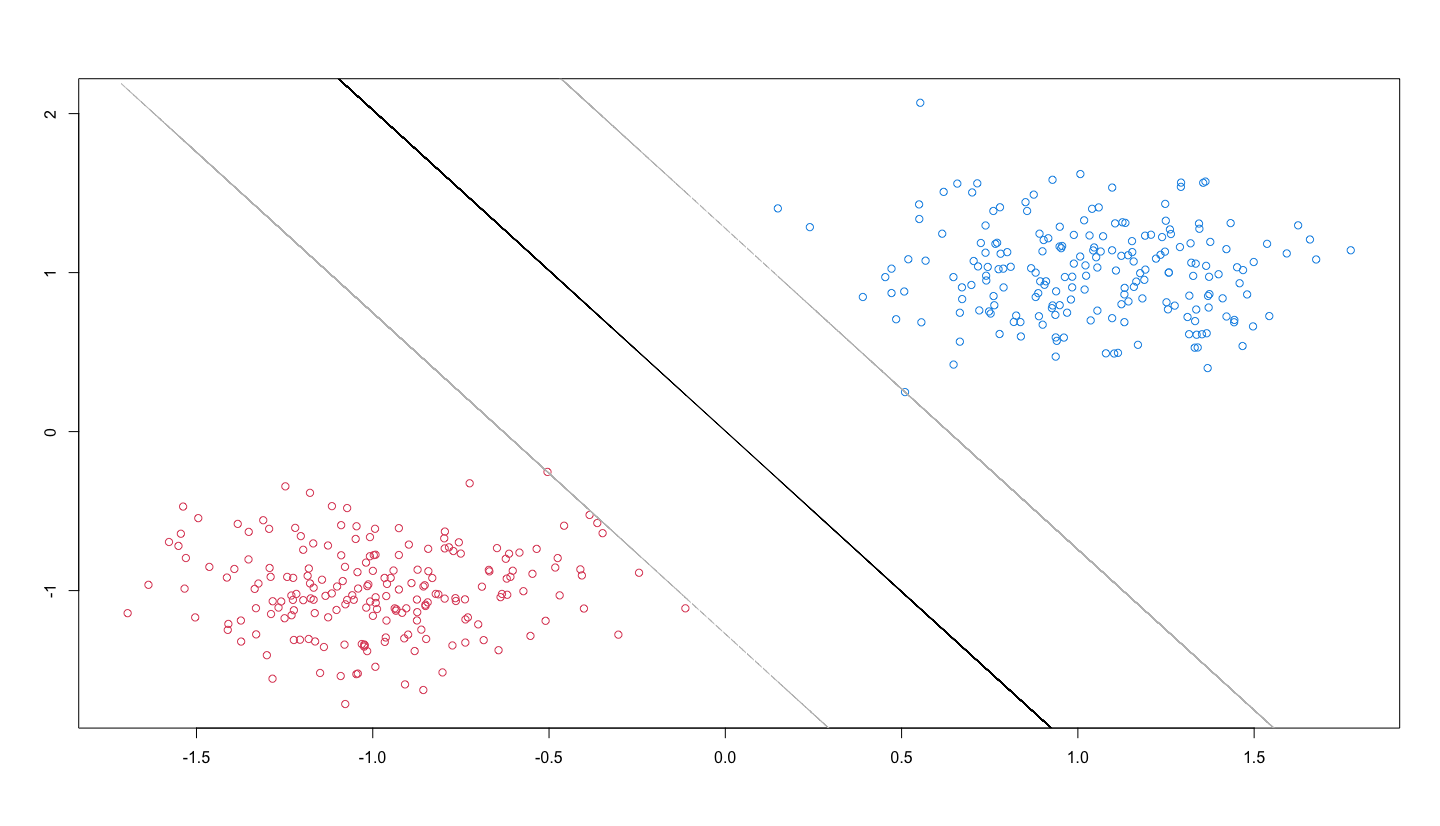
\includegraphics[width=5in]{Figures/mmc/mmc_graph.png}
    \caption{Maximal Margin Classifier Output in $R$}
    \label{fig_mmc_graph}
\end{figure}

To find the equation of the line, we use the hyperplane function as outlined in \cite{teitelbaum2021svm}:
\begin{minted}[breaklines]{R}
    hyperplane <- function(P,data,x,z=0) {
      alphas <- -1*P$coefs
      svs <- data[P$index,]
      c <- P$rho - z
      a <- sum(t(alphas)*data[P$index,][1])
      b <- sum(t(alphas)*data[P$index,][2])
      (-c-a*x)/b
    }
\end{minted}
In this function, \textbf{P} is the \textbf{svm} function which we labeled \textit{svmfit}. The \textbf{data} is our dataframe containing the observations and class labels. \textbf{x} is the column vector of observations. We set \textbf{z}=0 for now, but this will later be shown to move the hyperplane vertically by a set constant. 

Inside the function, the \textbf{alphas} are assigned to the coefficients of the hyperplane and multiplied by negative one. The \textbf{svs} variable takes the index of the support vectors and finds the exact point values in the data. \textbf{c} refers to the intercept and can be adjusted by the variable \textbf{z}. The variables \textbf{a} and \textbf{b} take the $x$ and $y$ coordinates, respectively, of the support vectors and multiply by their corresponding coefficient, as calculated by taking the transpose of the \textbf{alphas} variable, then summed. In Python, the \textbf{hyperplane} function looks slightly different due to the differences in the corresponding module, but the concept remains the same \cite{teitelbaum2021svm}.

\begin{minted}[breaklines]{Python}
    def hyperplane(P,x,z=0):
    """Given an SVC object P and an array of vectors x, computes the hyperplane wx+b=z"""
    alphas = P.dual_coef_
    svs = P.support_vectors_
    c = P.intercept_[0]-z
    a = np.sum(alphas.T*svs,axis=0)[0]
    b = np.sum(alphas.T*svs,axis=0)[1]
    return (-c-a*x)/b
\end{minted}

The $R$ code for the plot referenced in Figure ~\ref{fig_mmc_graph} is below and pulls information from the \textbf{hyperplane} function.

\begin{minted}[breaklines]{R}
    # set x and y variables into separate dataframes
    trainx <- cbind(train[,1],train[,2])
    trainy <- as.numeric(unlist(train[3]))
    
    # convert the y-values back to -1 and 1
    trainy[trainy == 1] <- -1
    trainy[trainy == 2] <- 1
    
    # calculating the hyperplane and supporting hyperplanes
    plt0 <- hyperplane(svmfit,train,trainx,0)
    plt1 <- hyperplane(svmfit,train,trainx,1)
    plt2 <- hyperplane(svmfit,train,trainx,-1)
    
    # plotting the data with hyperplanes
    plot(trainx,col=(3-trainy),xlab="",ylab="",pch=16)
    lines(trainx,plt0,col='black')
    lines(trainx,plt1,col='gray',lty='dashed')
    lines(trainx,plt2,col='gray',lty='dashed')
\end{minted}

Our discussion of the maximal margin classifier would not be complete without some sort of validation check. This is where the test set comes into play. We may now use our model to predict the class labels in the test set:

\begin{minted}[breaklines]{R}
    y_pred <- predict(svmfit, newdata = test[-3])
\end{minted}

The results can be viewed in a confusion matrix, which is a method of seeing true positives and negatives.

\begin{minted}[breaklines]{R}
    cm = table(test[,3], y_pred)
\end{minted}

The results are in Table ~\ref*{fig_mmc_cm}.

\begin{figure}[H]
    \centering
    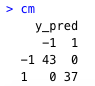
\includegraphics[width=1in]{Figures/mmc/mmc_cm.png}
    \caption{Maximal Margin Classifier Confusion Matrix}
    \label{fig_mmc_cm}
\end{figure}

From the zeroes along the diagonal in the top right and bottom left, we see there are no misclassified values. This is a good sign as our data is linearly separable!

\section{SUPPORT VECTOR CLASSIFIER}

What happens when data is not linearly separable? This occurs when the two groups of data have overlapping points. In this case, we cannot form a separating hyperplane as some points will be classified on the wrong side of the line. For non-linearly separable data, we introduce the support vector classifier. Much like the maximal margin classifier, we form a hyperplane between the groups of points in a data set. This classification method is also known as the soft-margin classifier since some points will not be classified on the correct side of the hyperplane unlike the maximal margin classifier. We will introduce the topic of costs, which essentially allow a certain number of observations to be classified incorrectly, then discuss the code in $R$ and Python.

The following code in $R$ can be used to plot non-linearly separable data with randomly generated points, shown in Figure ~\ref{fig_svc_randomly_generated_points}. We use the \textbf{set.seed()} function to replicate the randomly generated data. The process is the same as with linearly separable data, except we now narrow the gap between the means of the two groups which allows some overlap. Notice that we can no longer draw a straight line bisecting the two groups.

\begin{minted}[breaklines]{R}
    # setting initial number of observations
    n <- 200
    
    # calculating x-variable using two randomly generated sets with overlap
    set.seed(100)
    svcdatax1 <- matrix(rnorm(n*2, 0.5,0.3), ncol=2)
    svcdatax2 <- matrix(rnorm(n*2,-0.5,0.3), ncol=2)
    svcdatax <- rbind(svcdatax1,svcdatax2)
    
    # assigning labels to both classes
    svcdatay <- c(rep(-1,n), rep(1,n))
    
    # plotting the data
    plot(svcdatax, col=(3-svcdatay),xlab="",ylab="",pch=16)
\end{minted}

\begin{figure}
    \centering
    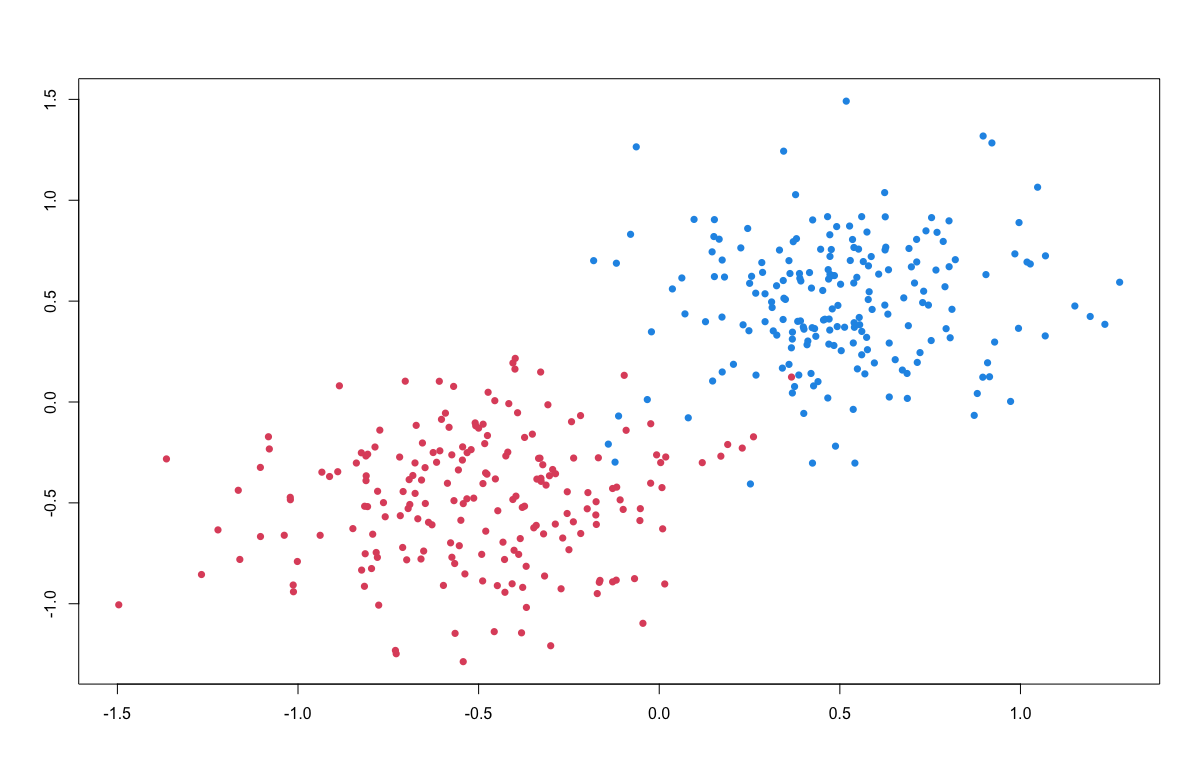
\includegraphics[width=5in]{Figures/svc/svc_randomly_generated_points.png}
    \caption{Randomly Generated Non-Linearly Separable Data}
    \label{fig_svc_randomly_generated_points}
\end{figure}

We can add a line to visualize a possible hyperplane by running the following line of code after we have constructed the graph.

\begin{minted}[breaklines]{R}
    abline(0,-1,col="gray",lty="dashed")
\end{minted}

\begin{figure}
    \centering
    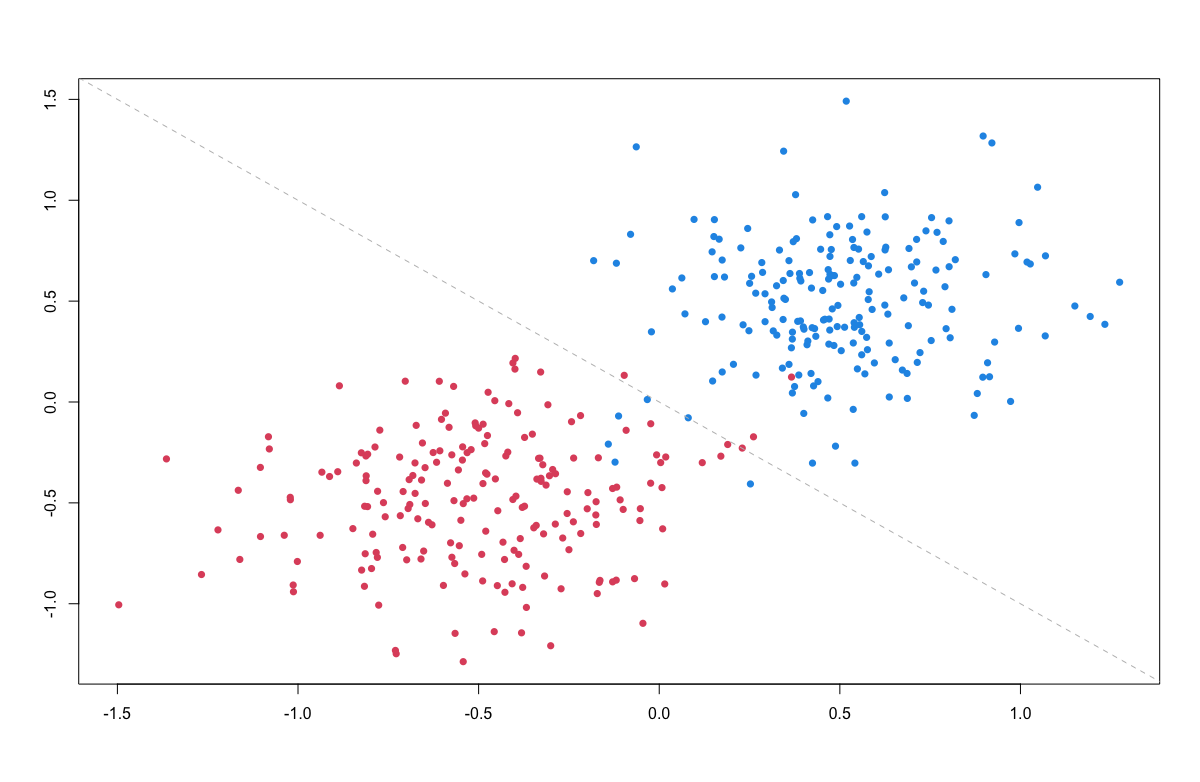
\includegraphics[width=5in]{Figures/svc/svc_randomly_generated_w_line.png}
    \caption{Randomly Generated Non-Linearly Separable Data With Line}
    \label{fig_svc_randomly_generated_w_line}
\end{figure}

As we can see, there is no possible linear hyperplane that separates the data. Some blue points are intermingled with the red and vice versa. To still construct a machine that attempts to classify the data, we introduce the topic of costs. In the maximal margin classifier, we aimed to find the greatest distance (margin) between the closest points of the two sets. Since there is no concrete margin in non-linearly separable data, we must introduce what is called a slack variable, denoted as $\epsilon_i$ for each observation $x_i$. For variables that are correctly classified, the corresponding observation's slack variable is 0. For points that are incorrectly classified, the slack variable takes on a value greater than 0 and incurs some cost for the maximization function. Since the slack variable is essentially a measure of how far a point lies on the wrong side of the margin, we constrict the sum of all slack variables to be less than a specified cost $C$. As we will see later, a user-defined cost can result in over- or under-fitting of the model. For a support vector classifier, the maximization of \(M\) is subject to \[ \sum_{j=1}^{p} \beta^2_j=1 \] \[ \sum_{i=1}^{n} \epsilon_i \le C, \epsilon_i \ge 0 \]

Let us introduce the concept of inner products and their role in the support vector classifier as outlined in \citep{introstatlearning} and \citep{esl2}. The inner products of two vectors is defined as \[ \langle a,b \rangle=\sum_{i=1}^{r}a_ib_i \] for two \(r\)-vectors \(a\) and \(b\). Following the work produced in \citep{introstatlearning}, the support vector classifier can be rewritten as \[f(x) = \beta_0 + \sum_{i=1}^n \alpha_i \langle x,x_i \rangle \] and the solution revolves around the inner products. Futhermore, it is known that each \(\alpha_i\) is non-zero only for the support vectors. The support vector classifier is simplified even more, as we can ignore points that are not support vectors. The solution then becomes \[f(x) = \beta_0 + \sum_{i \in S} \alpha_i \langle x,x_i \rangle \] provided that

\begin{equation}
\sum_{j=1}^{p} \beta^2_j=1
\end{equation}

\begin{equation} \label{slackvariables}
\sum_{i=1}^{n} \epsilon_i \le C, \epsilon_i \ge 0
\end{equation}

where \(S\) is the set of indices of the support vectors.

We now implement a support vector classifier in $R$. Using the same \textbf{svm} module as in the maximal margin classifier, we can find the best hyperplane to classify the data given a specified cost. We first create the dataframe and separate into a training and test set.

\begin{minted}[breaklines]{R}
    # creating data frame 
    svcdata <- data.frame (x = svcdatax, y = factor(svcdatay))
    
    # splitting into training and test data
    library(caTools)
    set.seed(100)
    
    # using 80% of the data in the training set and the other 20% in the test set
    sample <- sample.split(svcdata$x.1, SplitRatio = 0.8)
    train  <- subset(svcdata, sample == TRUE)
    test   <- subset(svcdata, sample == FALSE)
\end{minted}

Once we have split the data, we can compute the function using the training data. To begin we have specified the cost as 1000, but we will later discuss a better way to determine the best cost.

\begin{minted}[breaklines]{R}
    # computing svm function
    svmfit <- svm (y~., data = train , kernel="linear", cost = 1000, scale = FALSE)
    
    # looking at statistics
    summary(svmfit)
    svmfit$index
    svmfit$rho
    svmfit$coefs
    
    # plotting svm function graph
    plot(svmfit,train)
    
    # calculating the hyperplane and supporting hyperplanes
    plt0 <- hyperplane(svmfit,train,trainx,0)
    plt1 <- hyperplane(svmfit,train,trainx,1)
    plt2 <- hyperplane(svmfit,train,trainx,-1)
    
    # plotting the data with hyperplanes
    plot(trainx,col=(3-trainy),xlab="",ylab="",pch=16)
    lines(trainx,plt0,col='black')
    lines(trainx,plt1,col='gray')
    lines(trainx,plt2,col='gray')
    
\end{minted}

This produces the result in Figure ~\ref{fig_svc_data_w_hyperplanes}, graphically representing observations with slack variables greater than zero. Red points either inside the margin illustrated with the gray supporting hyperplanes or on the right side of the black hyperplane will have non-zero slack variables. Similarly, blue points inside the margin or on the left side of the hyperplane will have non-zero slack variables.

\begin{figure}[ht]
    \centering
    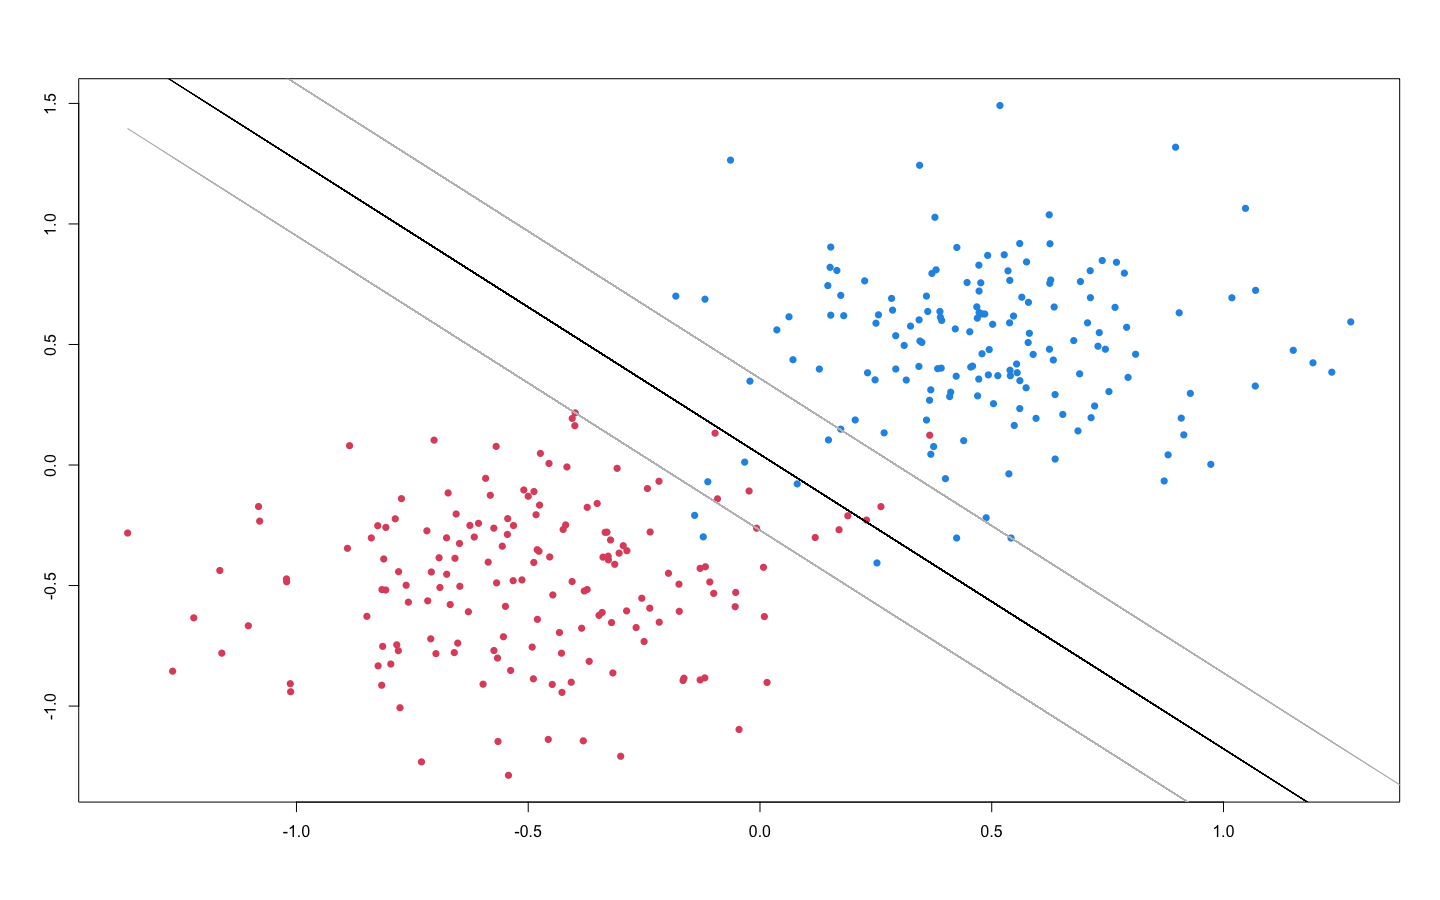
\includegraphics[width=5in]{Figures/svc/svc_data_w_hyperplanes.png}
    \caption{Randomly Generated Non-Linearly Separable Data With Line}
    \label{fig_svc_data_w_hyperplanes}
\end{figure}

Let us look at what happens with different values of the cost variable.

\begin{minted}[breaklines]{R}
    # using cost of 0.01
    svmfit01 <- svm (y~., data = train , kernel="linear", cost = .01, scale = FALSE)
    summary(svmfit01)
      # results in 224 support vectors
    
    # using cost of 1
    svmfit1 <- svm (y~., data = train , kernel="linear", cost = 1, scale = FALSE)
    summary(svmfit1)
      # results in 35 support vectors
    
    # using cost of 100
    svmfit100 <- svm (y~., data = train , kernel="linear", cost = 100, scale = FALSE)
    summary(svmfit100)
      # results in 21 support vectors
    
    # using cost of 1000
    svmfit1000 <- svm (y~., data = train , kernel="linear", cost = 1000, scale = FALSE)
    summary(svmfit1000)
      # results in 21 support vectors
\end{minted}

We see that as the cost increases, there are fewer support vectors. That is, fewer observations are classified incorrectly. Shouldn't it be the opposite? We see in ~\ref{slackvariables} that the sum of the slack variables has to be less than or equal to the cost. A higher cost allows for greater slack variables, meaning more observations can lie outside the margin. This discrepancy lies in the underlying code. In both the R and Python modules for the support vector machine, the cost is inversely proportional to the \(C\) we defined in ~\ref{slackvariables}.

The difference is a reference to the "dual problem", as there are two approaches to solving this problem. One approach, which we have previously outlined, fixes the variable \(C\) and the sum of \(\beta_j^2\) in order to minimize the margin. We are left with solving \[
    y_i(\beta_0+\beta_1x_{i1}+...+\beta_px_{ip}) \ge M(1-\epsilon_i)
    \]
subject to the conditions on \(\beta\) and \(\epsilon\). We could also solve this problem by switching our conditions and minimization as outlined in \cite{esl2}. If we fix the margin to be 1, we aim to minimize \(||\beta||\). The new problem becomes 

\begin{equation} 
    \min ||\beta|| \text{ subject to }
    \begin{cases}
        &y_i(\beta x_i + \beta_0) \ge 1 - \epsilon_i \forall i, \\ & \epsilon_i \ge 0, \sum \epsilon_i \le \text{constant} 
    \end{cases}
    \label{eq_svc_initial}
\end{equation}

which is equivalent to

\begin{equation}
    \begin{cases}
        & \min_{\beta,\beta_0} \frac{1}{2} ||\beta||^2 + C \sum_{i=1}^{N} \epsilon_i \\
        & \text{subject to } y_i(\beta_i x_i^T+\beta_0) \ge 1 - \epsilon_i, \epsilon_i \ge 0
    \end{cases}
    \label{eq_svc_final}
\end{equation}

The constant defined in ~\ref{eq_svc_initial} is replaced with the cost parameter of the Lagrange function in ~\ref{eq_svc_final}. This cost parameter is the same as the variable defined in both the $R$ and Python $\textbf{svm}$ modules.

We saw that choosing different costs affects the number of support vectors. A smaller cost results in a lower penalty for each misclassified data point. As such, the resulting margin is large. When the cost is larger, misclassified data points have a bigger impact on the model, so the resulting margin is smaller to minimize these points \citep{cost_parameter}. How does one go about determining the correct cost though? Luckily, the $\textbf{svm}$ function can be used in a $\textbf{tuning}$ function that tests various costs for the correlating model accuracy. We use the following code to determine the best model:

\begin{minted}[breaklines]{R}
    # tune the function to find the best model with various costs
    tune <- tune(svm, y~., data = train, 
                 ranges = list(cost = 2^(-2:10)), tunecontrol = tune.control(sampling = "fix"))
    
    # we see a cost of 0.25 gives the best model
    tune$best.parameters
    
    # calculating the model error
    tune$best.performance
\end{minted}

We can again validate our model using the test set. The same code as covered in the maximal margin classifier is used, and we see there are no misclassified points. Thus, we have produced the best support vector classifier for our data, illustrated in Figure ~\ref{fig_svc_final_model}.

\begin{figure}[ht]
    \centering
    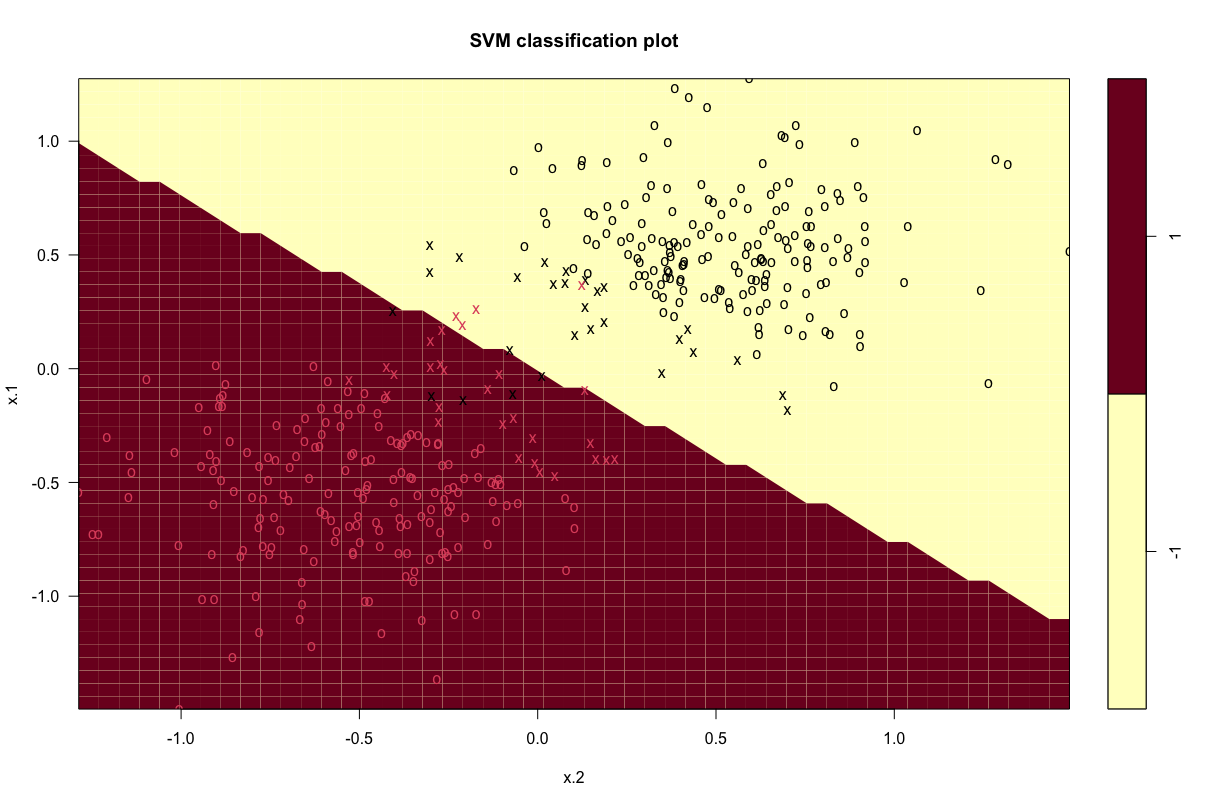
\includegraphics[width=5in]{Figures/svc/svc_final_model.png}
    \caption{Final SVC Model with \(C = 0.25\)}
    \label{fig_svc_final_model}
\end{figure}

\section{SUPPORT VECTOR MACHINES}

Previously, we have only worked with data involving two classes. The maximal margin classifier is used for linearly separable data, and the support vector classifier is used for non-linearly separable data. When there are more than two classes, a support vector machine is used. A linear hyperplane is not appropriate for multi-class data, so we introduce the concept of a kernel.

Recall the inner products from the support vector classifier. The kernel is a generalized representation of the inner product of two observations \[K(x_i,x_i')\] where \(K\) is some function that measures the similarity between two observations \citep{introstatlearning}. In the support vector classifier, the kernel is a linear function calculated using Pearson correlation. For non-linear data, this function \(K\) can be replaced with another form. Common quantities include

\begin{center}
    \begin{tabular}{c|c}
        \(K\) & Form \\
        \hline \\
        linear & \(\sum_{j=1}^p x_{ij}x_{i'j}\) \\
          \\

        polynomial & \((1+ \sum_{j=1}^p x_{ij}x_{i'j})^d \) \\
          \\

        radial & \(\exp ( - \gamma \sum_{j=1}^p (x_{ij}-x_{i'j})^2) \)
    \end{tabular}
\end{center}

We will focus on the radial kernel. The radial kernel is a popular first choice as it performs well in multi-class data with a non-linear relationship. In addition to the cost parameter, we now have the gamma parameter. Common choices for the cost parameter range from \(2^{-5}\) to \(2^{15}\) and for the gamma parameters range from \(2^{-15}\) to \(2^{3}\). One can input these ranges into the \textbf{tune} function to determine the best performing values for the model.

To implement this in $R$, we first create randomly generated multi-class data with the following code:

\begin{minted}[breaklines]{R}
    # setting initial number of observations in each set
    n <- 200

    # calculating x-variable using three randomly generated sets with overlap
    set.seed(1000)

    svmdatax1a <- matrix(rnorm(n, 0.25,0.3), ncol=1)
    svmdatax1b <- matrix(rnorm(n,0.75,0.3), ncol=1)
    svmdatax1 <- cbind(svmdatax1a,svmdatax1b)

    svmdatax2 <- matrix(rnorm(n*2,-0.5,0.4), ncol=2)

    svmdatax3a <- matrix(rnorm(n,1.5,0.3), ncol=1)
    svmdatax3b <- matrix(rnorm(n,1,0.3), ncol=1)
    svmdatax3 <- cbind(svmdatax3a,svmdatax3b)

    svmdatax <- rbind(svmdatax1,svmdatax2,svmdatax3)

    # assigning labels to both classes
    svmdatay <- c(rep(1,n), rep(2,n), rep(3,n))

    # plotting the data
    plot(svmdatax, col=(11-svmdatay),xlab="",ylab="",pch=16)
\end{minted}

Data can look like that in Figure ~\ref{fig_svm_randomly_generated_data}.

\begin{figure}[ht]
    \centering
    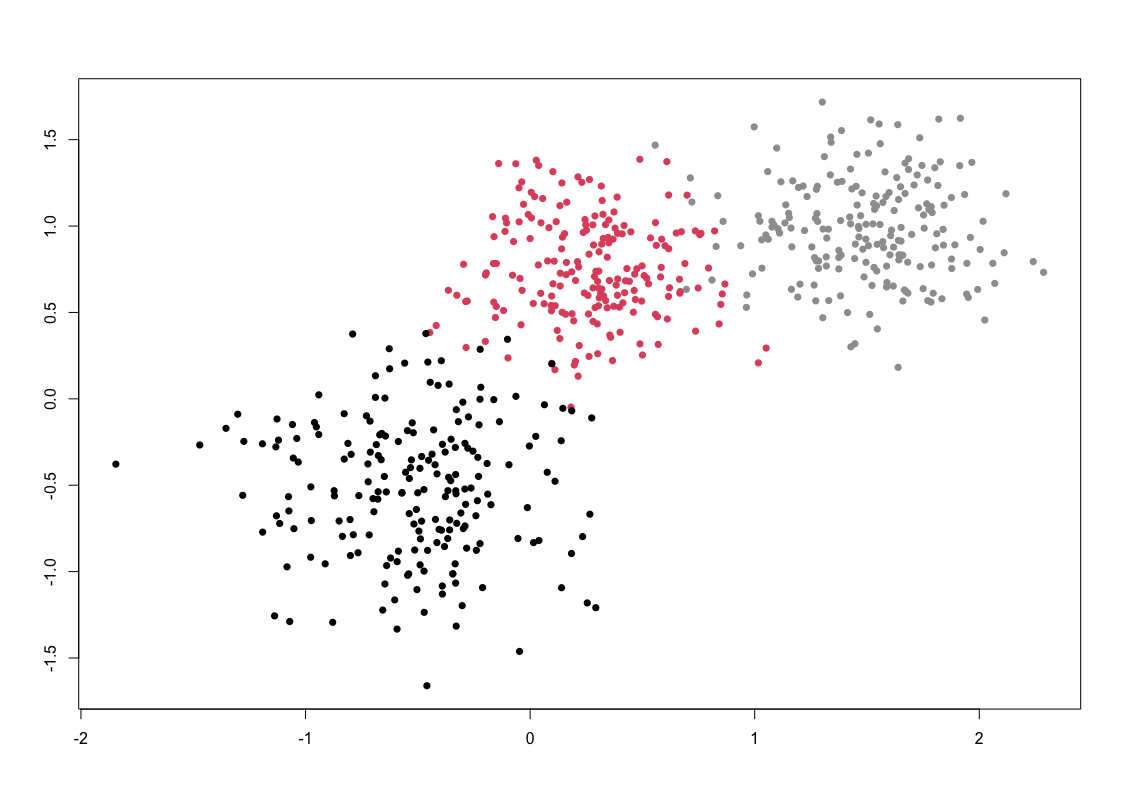
\includegraphics[width=5in]{Figures/svm/svm_randomly_generated_data.png}
    \caption{Randomly Generated Multi-Class Data}
    \label{fig_svm_randomly_generated_data}
\end{figure}

We now create the dataframe and split into training and test sets.

\begin{minted}[breaklines]{R}
    # creating data frame 
    svmdata <- data.frame (x = svmdatax, y = factor(svmdatay))
    
    # splitting into training and test data
    library(caTools)
    set.seed(100)
    
    # using 80% of the data in the training set and the other 20% in the test set
    sample <- sample.split(svmdata$x.1, SplitRatio = 0.8)
    train  <- subset(svmdata, sample == TRUE)
    test   <- subset(svmdata, sample == FALSE)    
\end{minted}

Now we are ready to run the \textbf{svm} module on our data. We previously discussed the importance of choosing a cost in the support vector classifier. What happens if we change the cost for a non-linear dataset? We will compute the support vector machine below using different cost values and compare.

\begin{minted}[breaklines]{R}
    # using different costs
    svmfit.001 <- svm (y~., data = train , kernel="radial", cost = 0.001, scale = FALSE)
    svmfit.1 <- svm (y~., data = train , kernel="radial", cost = 0.1, scale = FALSE)
    svmfit1 <- svm (y~., data = train , kernel="radial", cost = 1, scale = FALSE)
    svmfit1000 <- svm (y~., data = train , kernel="radial", cost = 1000, scale = FALSE)
    svmfit100000 <- svm (y~., data = train , kernel="radial", cost = 100000, scale = FALSE)
    svmfit10000000 <- svm (y~., data = train , kernel="radial", cost = 10000000, scale = FALSE)
    
    # plots of different costs
    plot(svmfit.001,svmdata,color.palette = terrain.colors,symbolPalette = c("red","black","darkgray"))
    plot(svmfit.1,svmdata,color.palette = terrain.colors,symbolPalette = c("red","black","darkgray"))
    plot(svmfit1,svmdata,color.palette = terrain.colors,symbolPalette = c("red","black","darkgray"))
    plot(svmfit1000,svmdata,color.palette = terrain.colors,symbolPalette = c("red","black","darkgray"))
    plot(svmfit100000,svmdata,color.palette = terrain.colors,symbolPalette = c("red","black","darkgray"))
    plot(svmfit10000000,svmdata,color.palette = terrain.colors,symbolPalette = c("red","black","darkgray"))
\end{minted}

The code produces the graphs in Figure ~\ref{fig_svm_diff_costs}. Initially, with a low cost every point is a support vector. In fact, the machine does not even distinguish between the various groups. In a dataset with 600 observations, 600 support vectors is not ideal. This makes sense, as a smaller cost means a lower penalty for each misclassified data point. As we increase the cost parameter, the number of support vectors decreases because the cost of being misclassified is greater. At the highest cost of 10,000,000 there are only 35 support vectors. We see a trade-off between the number of observations that influence the support vector machine and the associated cost. Zooming in, the support vectors in ~\ref{fig_svm_diff_costs} are labeled with an "x".

\begin{figure}[H]
    \centering
    \begin{align*}
    & C=0.001 & C=0.1 \\
    & 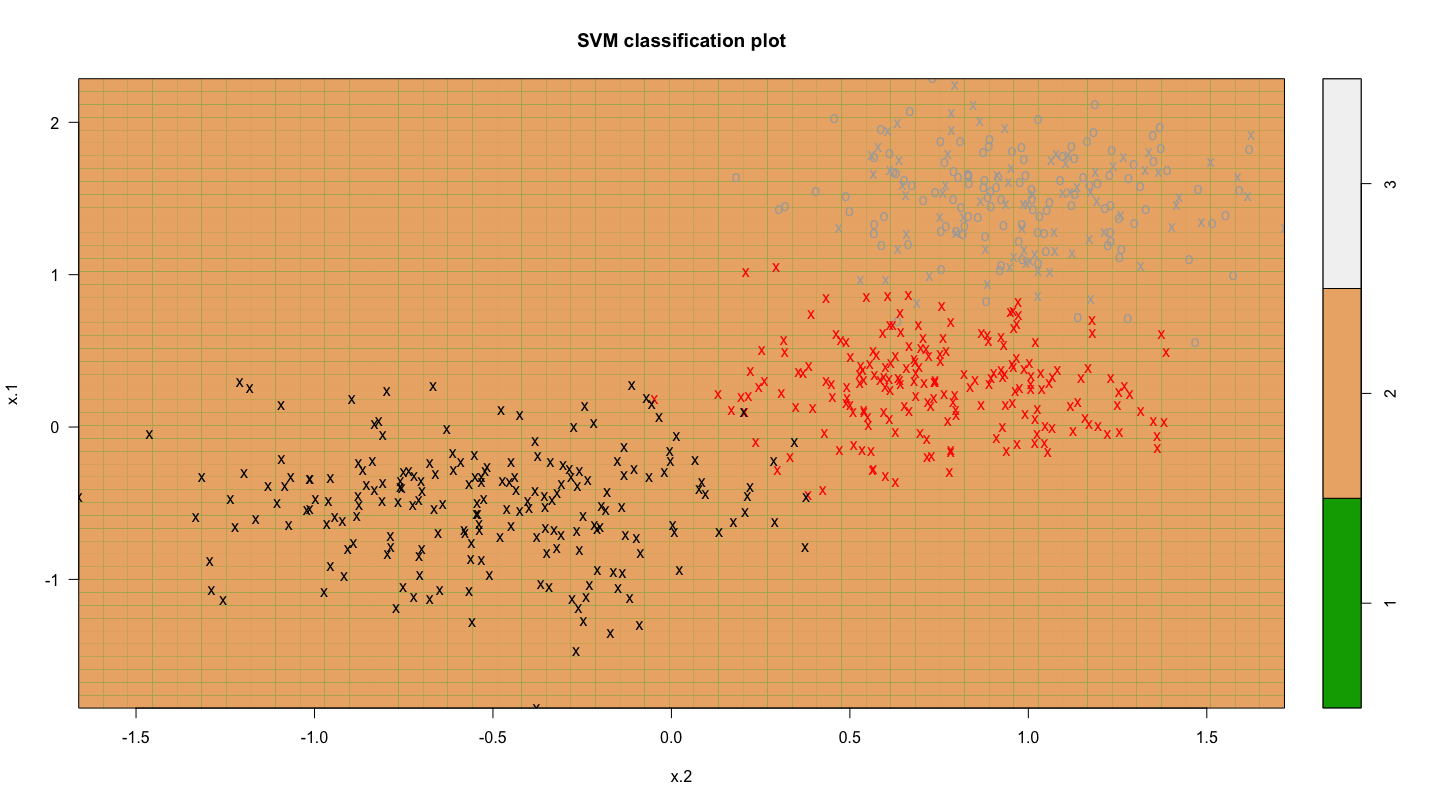
\includegraphics[width=3in]{Figures/svm/svm.001.png} &
    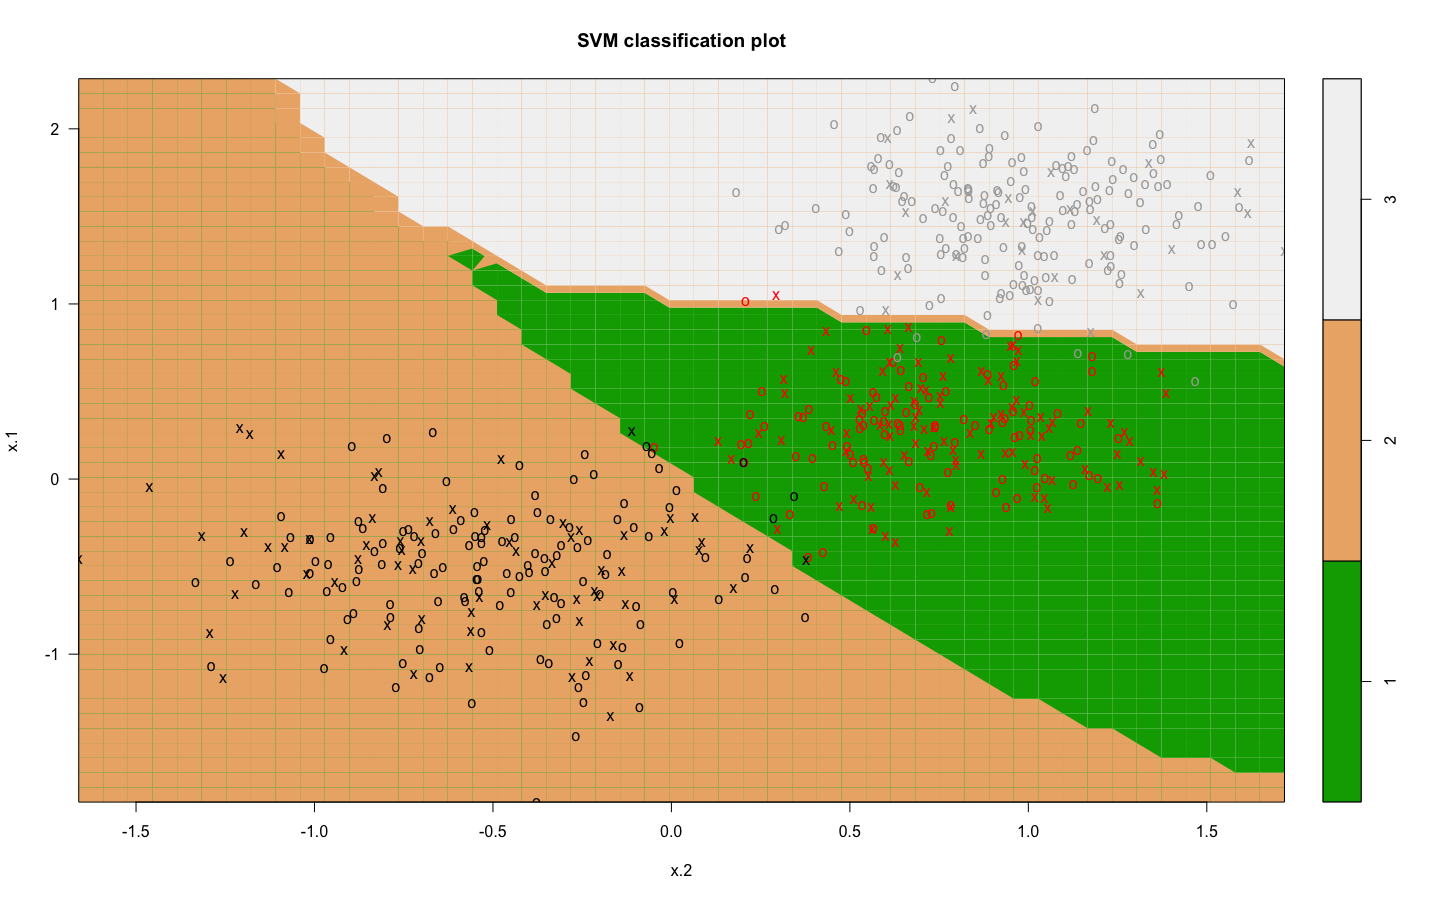
\includegraphics[width=3in]{Figures/svm/svm.1.png} \\
    & C=1 & C=1000 \\
    & 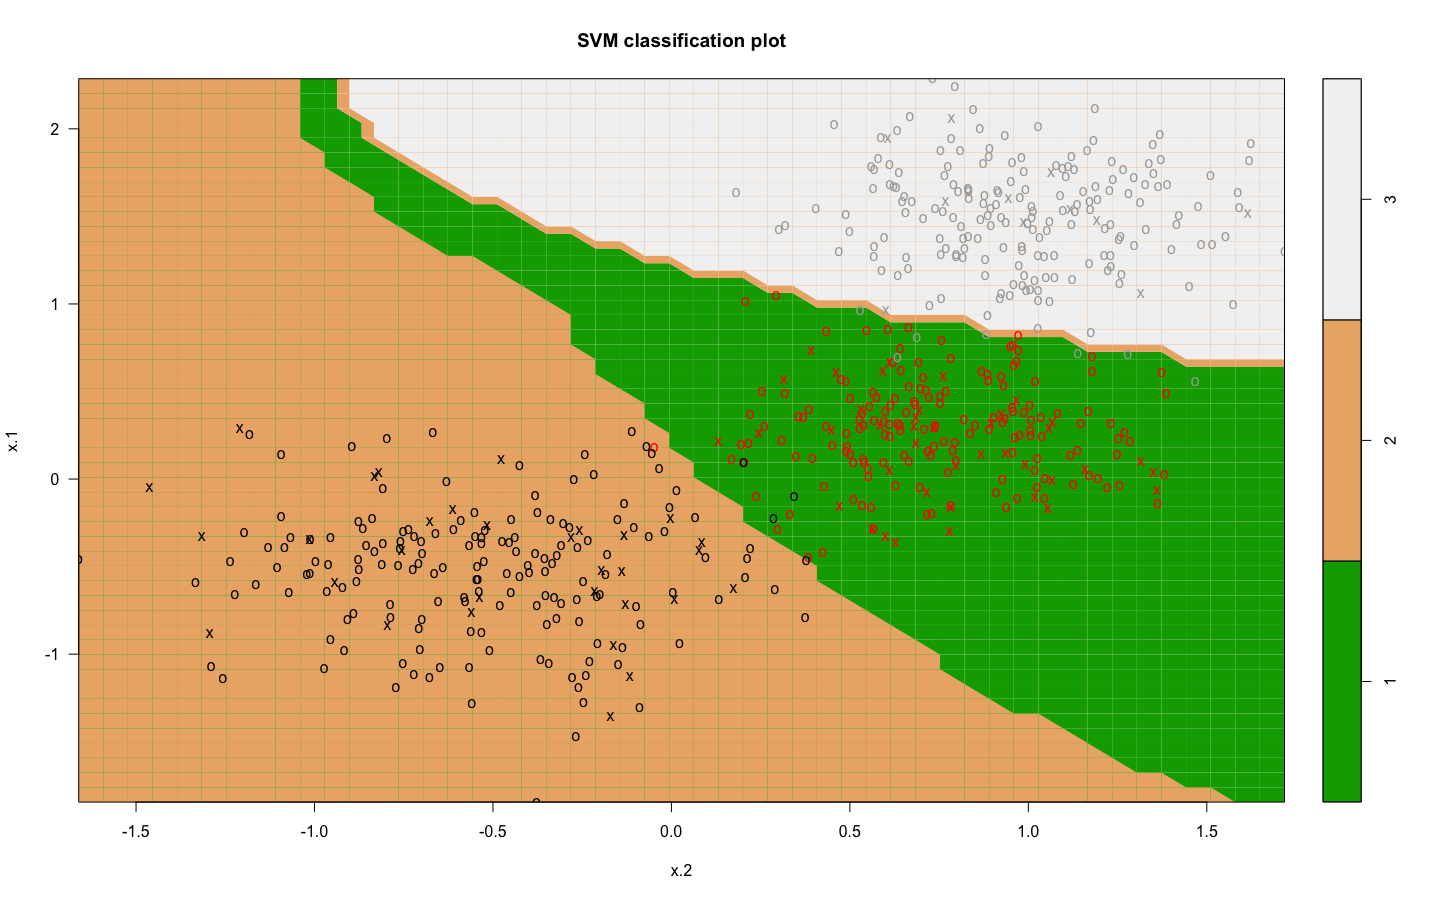
\includegraphics[width=3in]{Figures/svm/svm1.png} &
    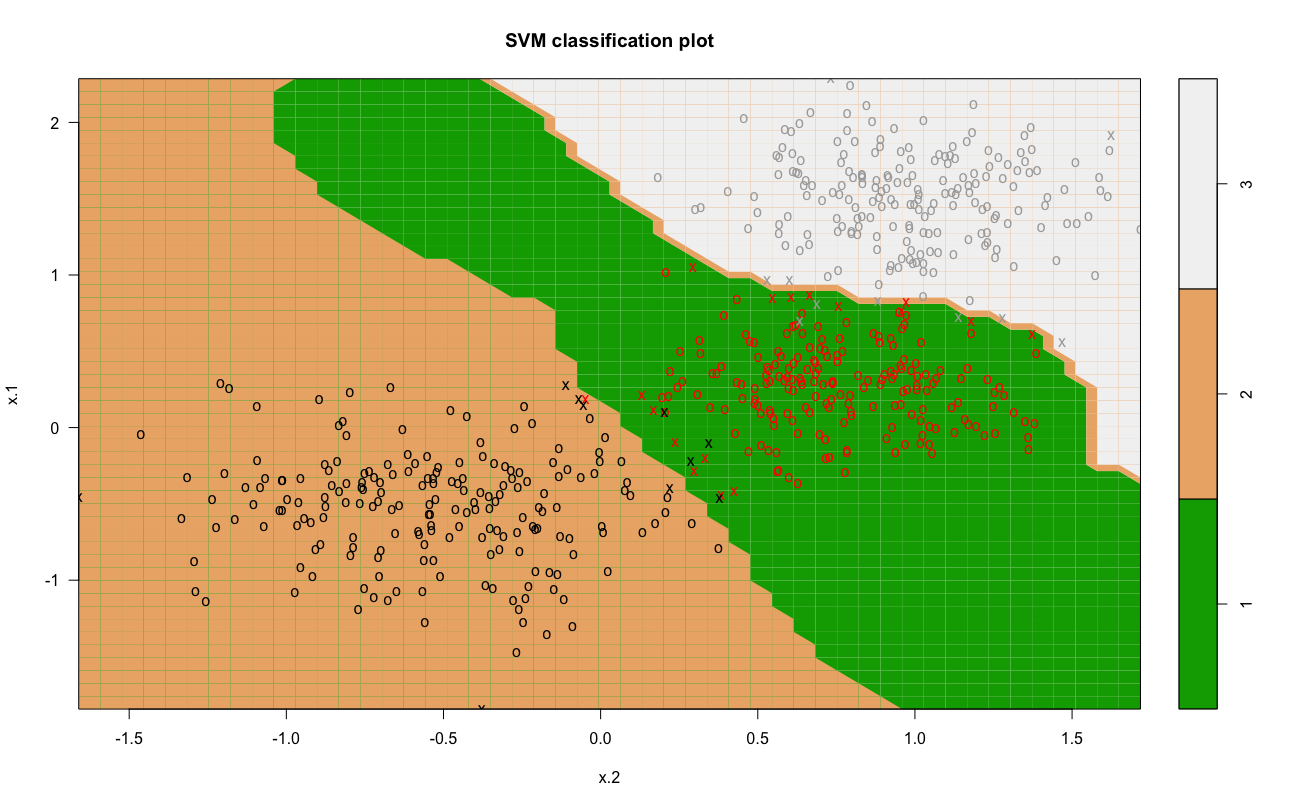
\includegraphics[width=3in]{Figures/svm/svm1000.png} \\
    & C=100000 & C=10000000 \\
    & 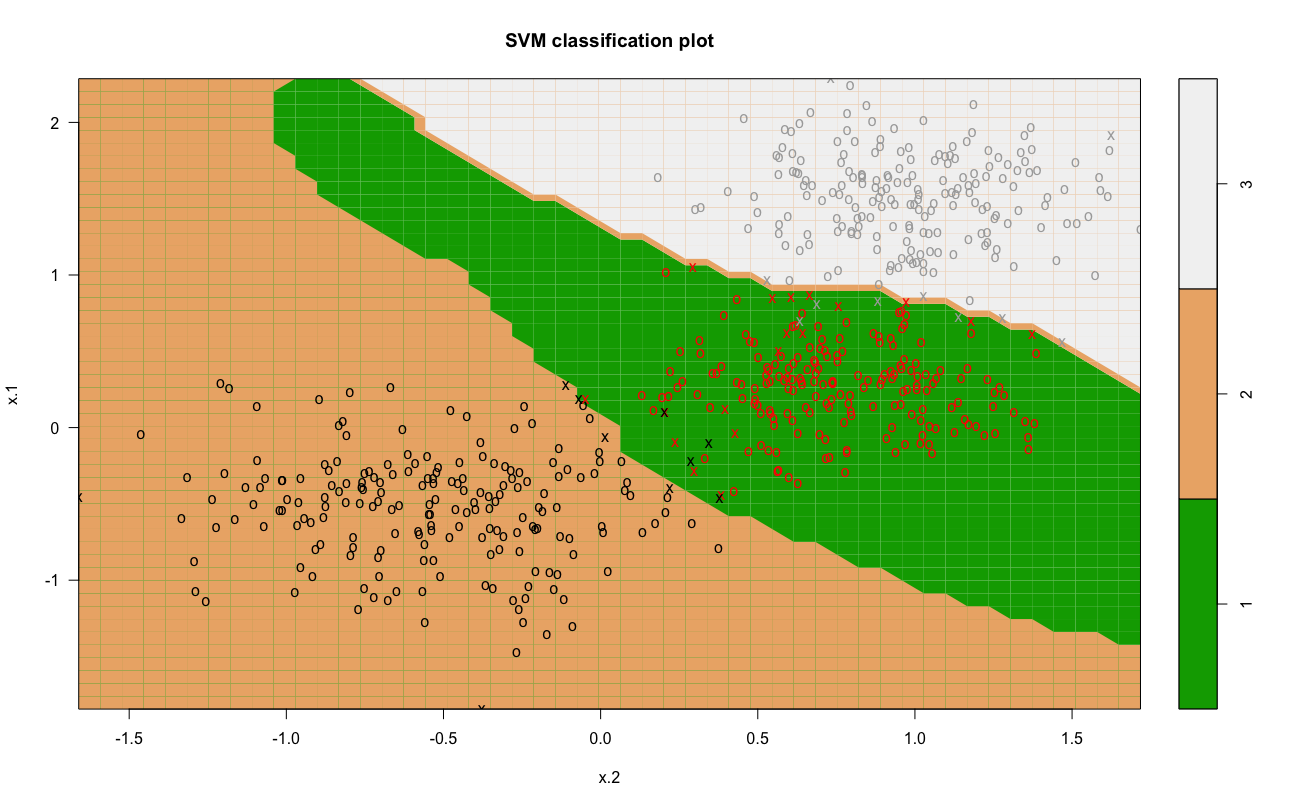
\includegraphics[width=3in]{Figures/svm/svm100000.png} &
    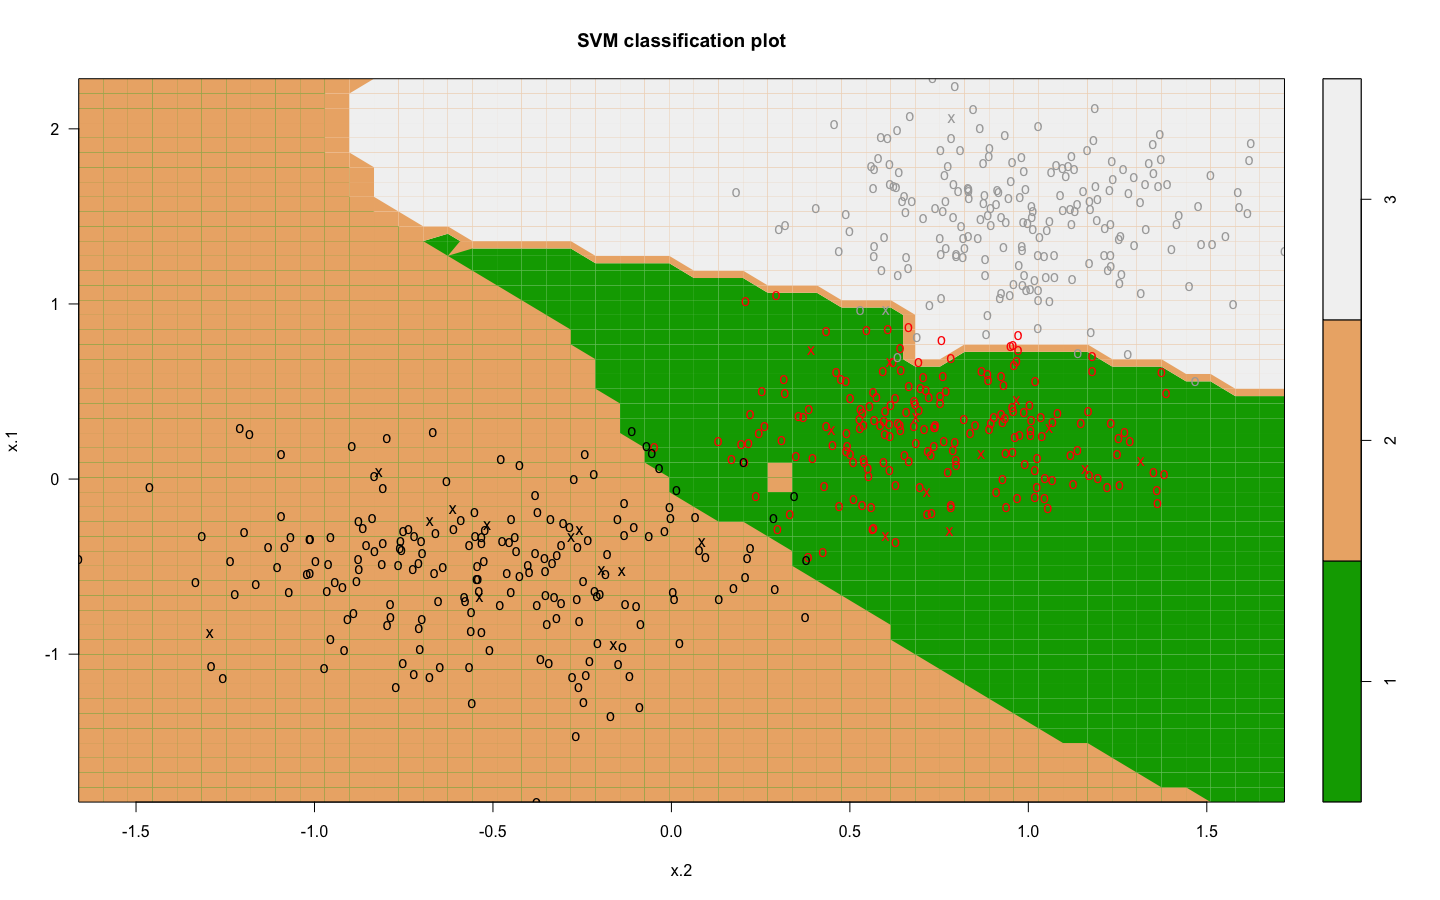
\includegraphics[width=3in]{Figures/svm/svm1000000.png}
    \end{align*}
    \caption{Experimentation with Different Costs in Non-Linear Data}
    \label{fig_svm_diff_costs}
\end{figure}

What happens if we change the gamma value? We try below with different values and compare.

\begin{minted}[breaklines]{R}
    # using different gammas
    svmfit.01g <- svm (y~., data = train , kernel="radial", cost = 1, gamma = 0.01, scale = FALSE)
    svmfit.1g <- svm (y~., data = train , kernel="radial", cost = 1, gamma = 0.1, scale = FALSE)
    svmfit1g <- svm (y~., data = train , kernel="radial", cost = 1, gamma = 1, scale = FALSE)
    svmfit10g <- svm (y~., data = train , kernel="radial", cost = 1, gamma = 10, scale = FALSE)
    svmfit100g <- svm (y~., data = train , kernel="radial", cost = 1, gamma = 100, scale = FALSE)
    svmfit1000g <- svm (y~., data = train , kernel="radial", cost = 1, gamma = 1000, scale = FALSE)
    
    # plots of different gammas
    plot(svmfit.01g,svmdata,color.palette = terrain.colors,symbolPalette = c("red","black","darkgray"))
    plot(svmfit.1g,svmdata,color.palette = terrain.colors,symbolPalette = c("red","black","darkgray"))
    plot(svmfit1g,svmdata,color.palette = terrain.colors,symbolPalette = c("red","black","darkgray"))
    plot(svmfit10g,svmdata,color.palette = terrain.colors,symbolPalette = c("red","black","darkgray"))
    plot(svmfit100g,svmdata,color.palette = terrain.colors,symbolPalette = c("red","black","darkgray"))
    plot(svmfit1000g,svmdata,color.palette = terrain.colors,symbolPalette = c("red","black","darkgray"))
\end{minted}

The code produces the graphs in Figure ~\ref{fig_svm_diff_gammas}. From \cite{scikit_rbf_parameters}, the "gamma parameter defines how far the influence of a single training example reaches, with low values meaning ‘far’ and high values meaning ‘close’." With the lowest gamma value of 0.01, the support vector machine mostly consists of straight lines as the influence of individual support vectors reaches farther out. As we increase the gamma value, the machine becomes more specialized to the dataset. We see the gamma value of 1000 yields a model with 600 out of the 600 points being support vectors. Each point has only a small radius of influence, leading to an extremely localized model with margins closely following the class boundaries. Choosing an appropriate gamma value helps protect against under- and over-fitting the model.

\begin{figure}[H]
    \centering
    \begin{align*}
    & \gamma=0.01 & \gamma=0.1 \\
    & 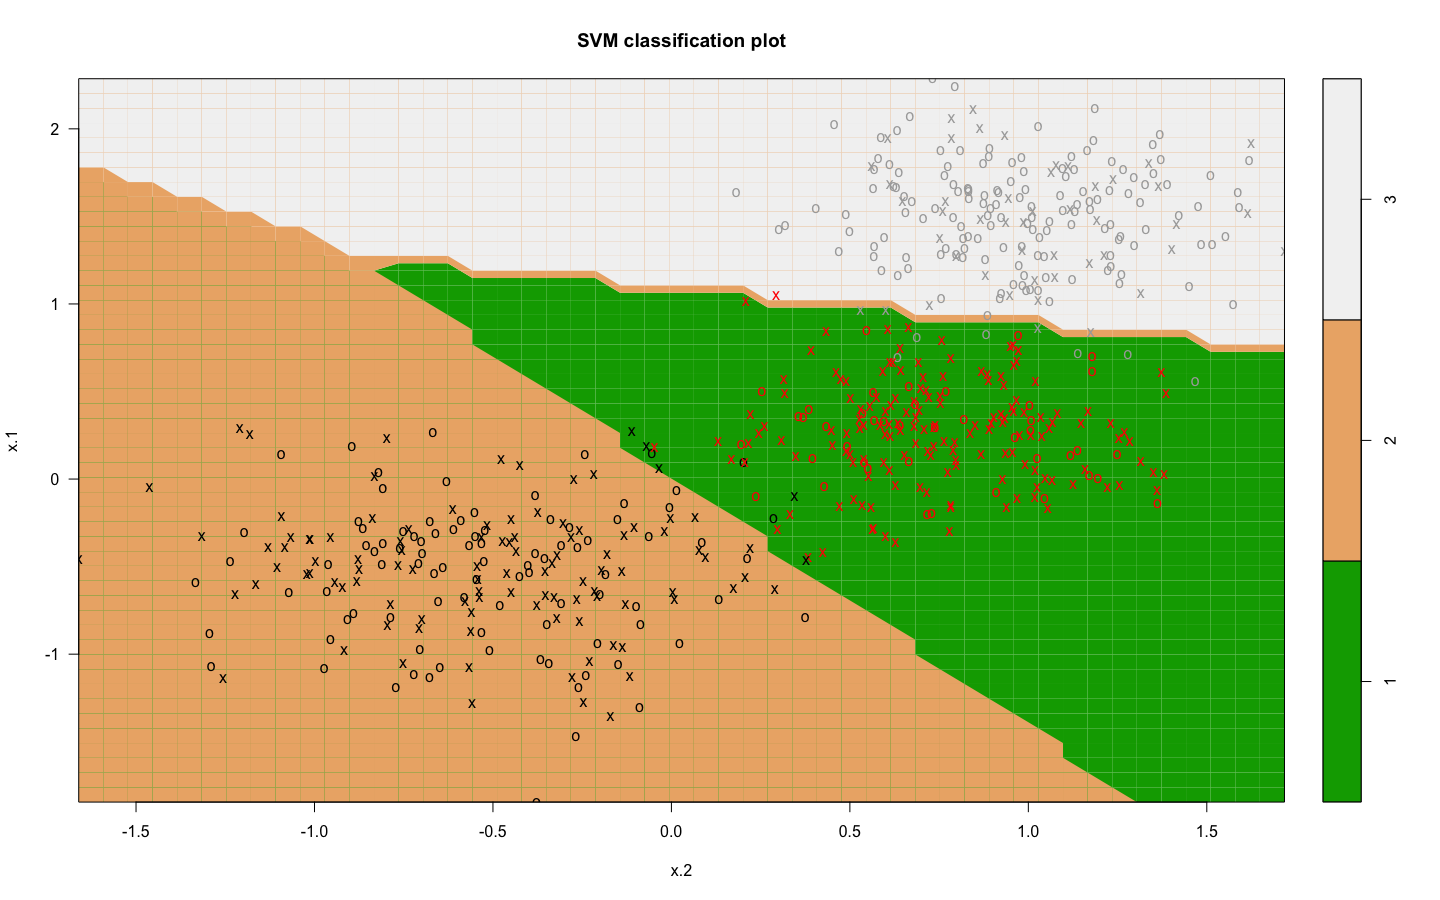
\includegraphics[width=3in]{Figures/svm/svmfit.01g.png} &
    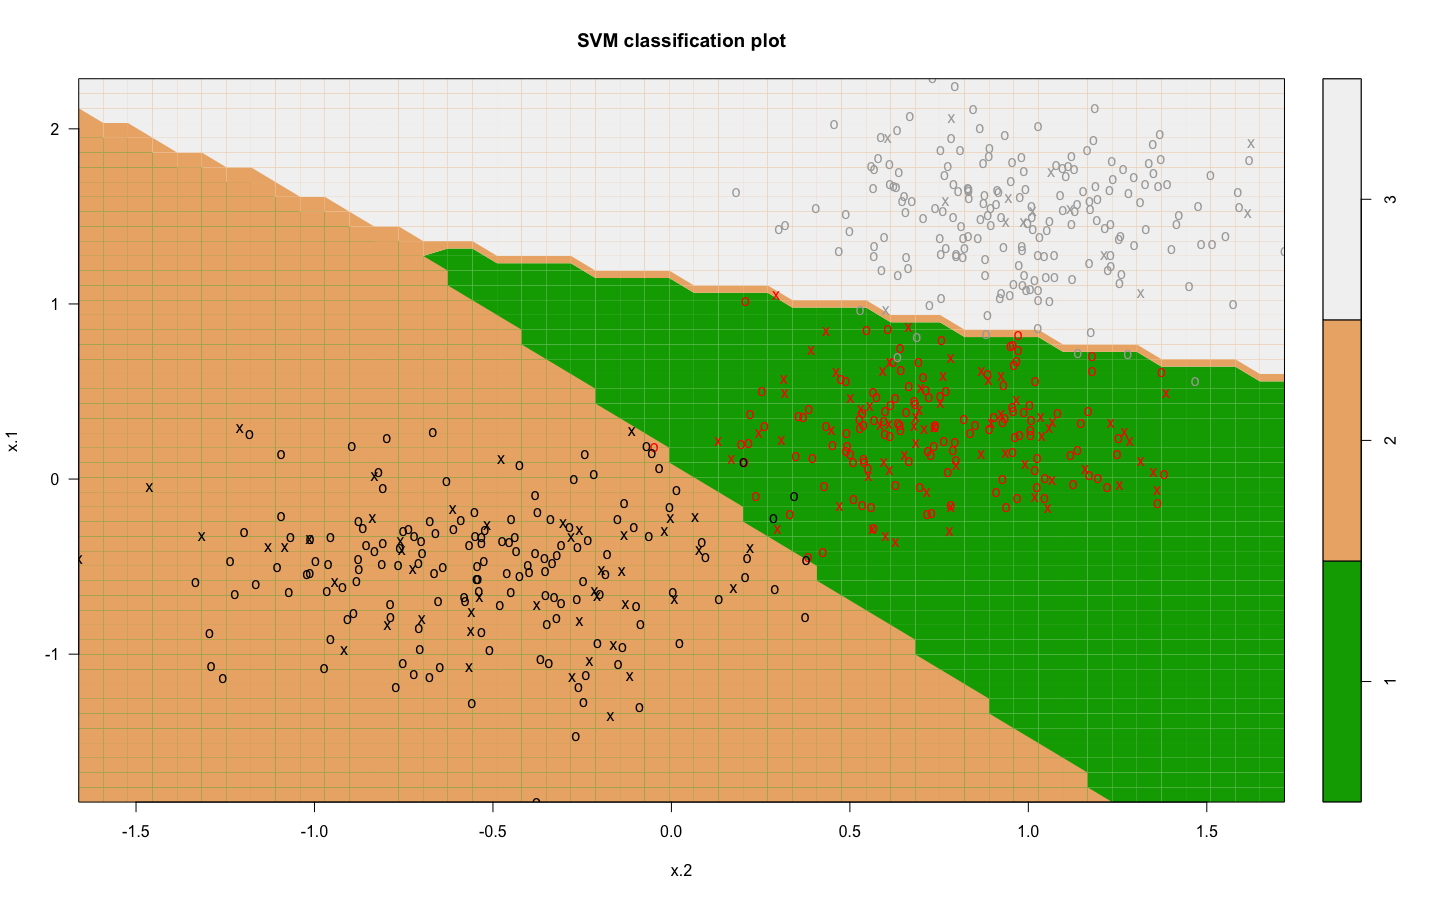
\includegraphics[width=3in]{Figures/svm/svmfit.1g.png} \\
    & \gamma=1 & \gamma=10 \\
    & 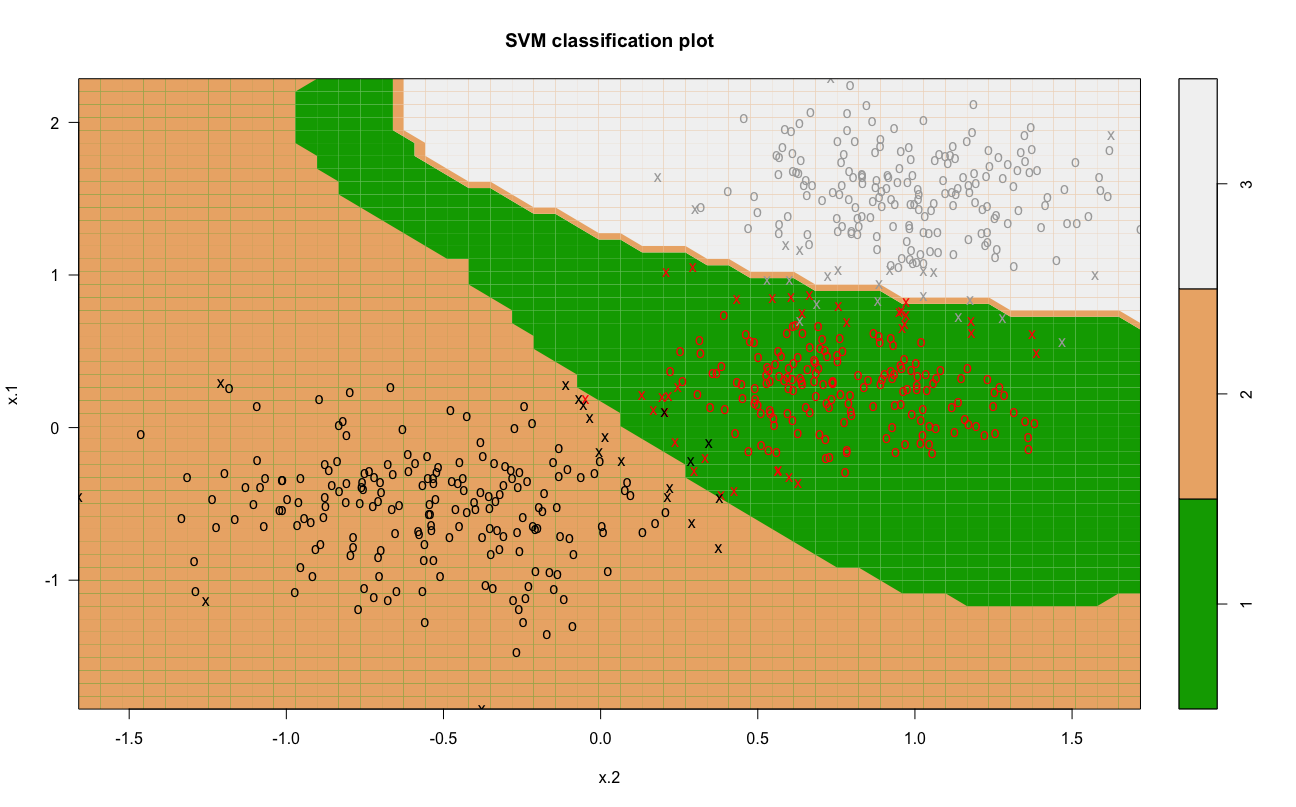
\includegraphics[width=3in]{Figures/svm/svmfit1g.png} &
    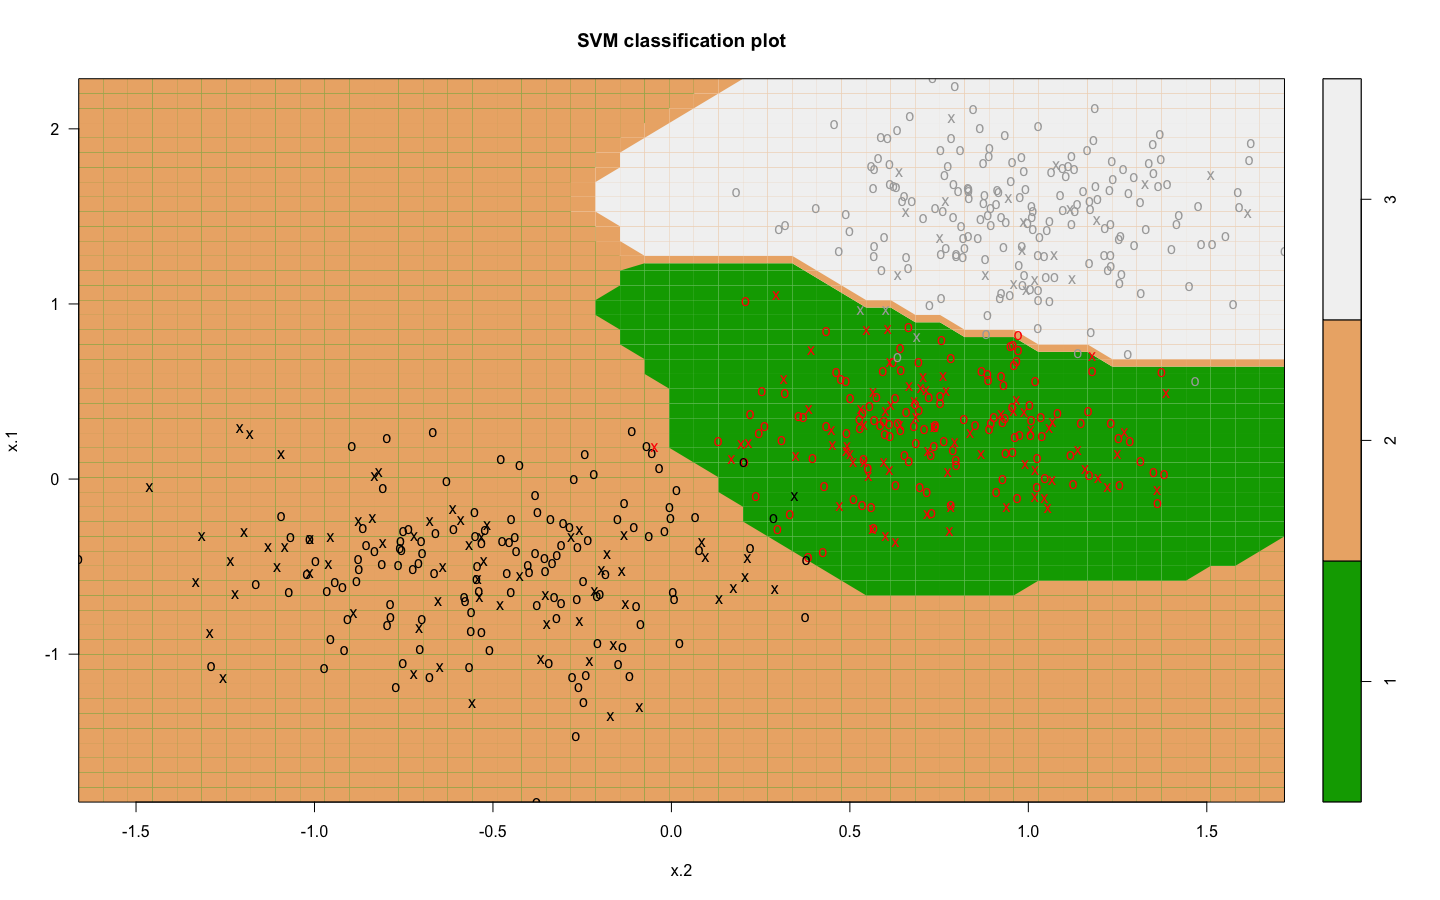
\includegraphics[width=3in]{Figures/svm/svmfit10g.png} \\
    & \gamma=100 & \gamma=1000 \\
    & 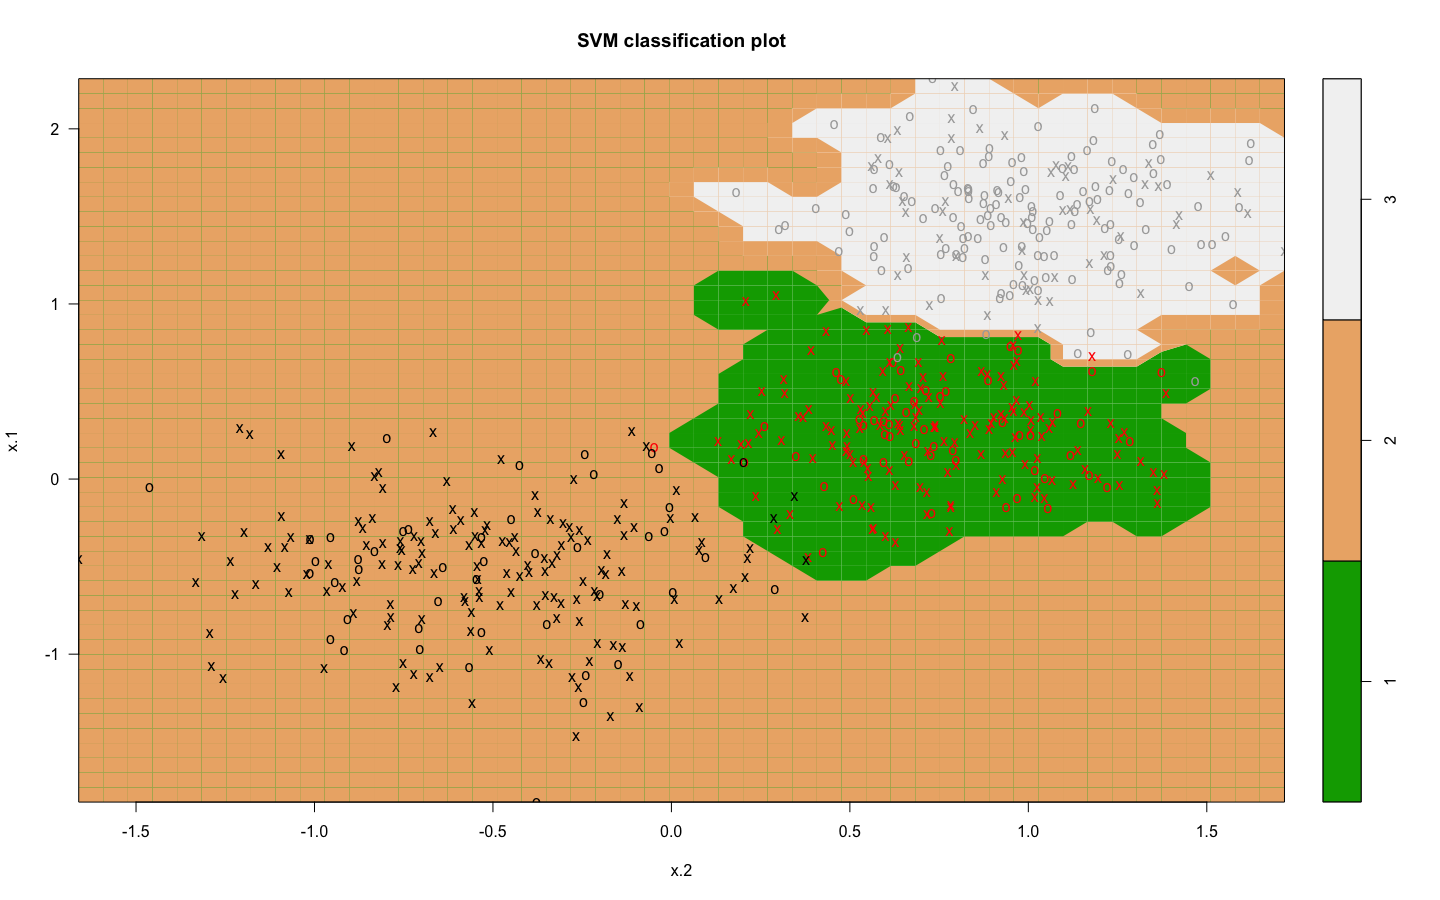
\includegraphics[width=3in]{Figures/svm/svmfit100g.png} &
    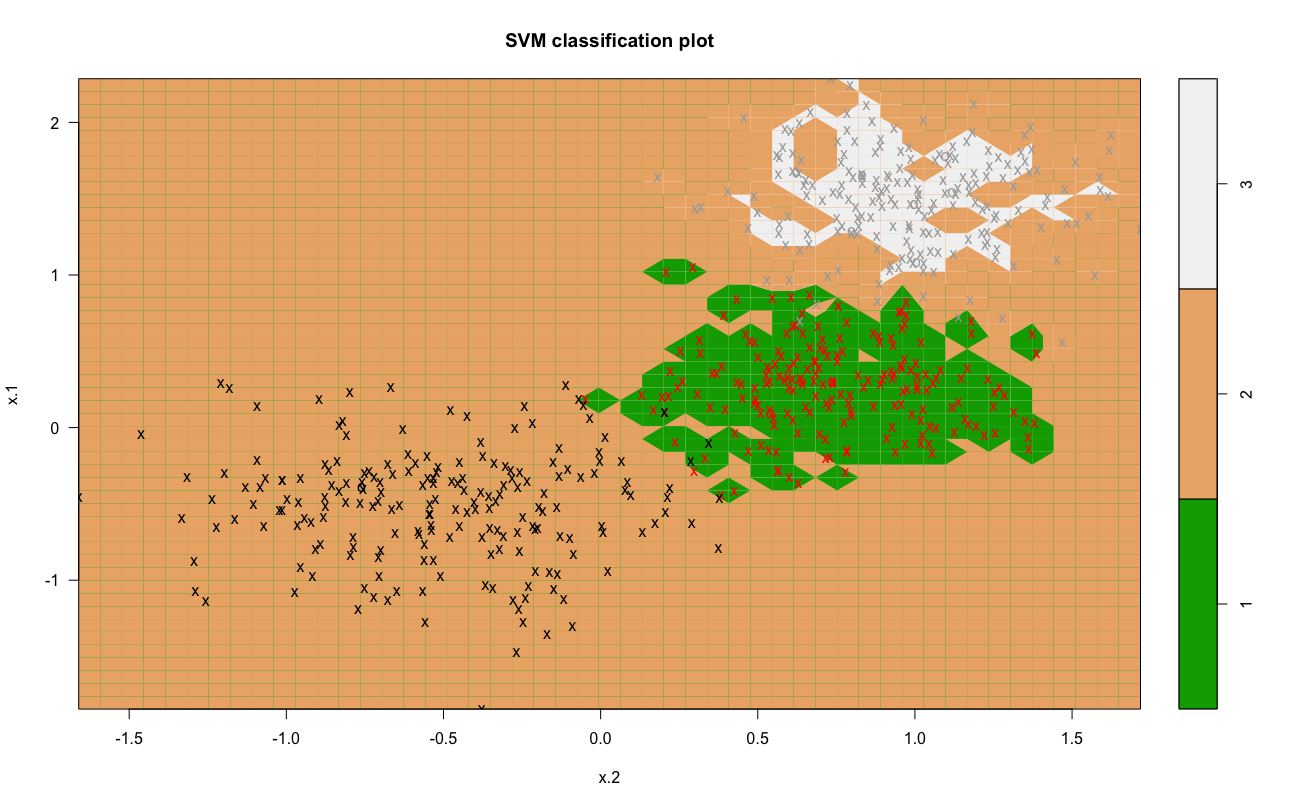
\includegraphics[width=3in]{Figures/svm/svmfit1000g.png}
    \end{align*}
    \caption{Experimentation with Different Gammas in Non-Linearly Separable Data}
    \label{fig_svm_diff_gammas}
\end{figure}

Using the tuning parameter, we can determine the best values for the cost and gamma parameters based on the lowest error. This helps increase the accuracy and validity of the model.

\begin{minted}[breaklines]{R}
    # using tune function to find the best model
    tune <- tune(svm, y~., data = train, 
                 ranges = list(gamma = c(2^(-2:10),1^(-2:10)), cost = c(2^(-2:10),1^(-2:10))), tunecontrol = tune.control(sampling = "fix"))
    
    tune$best.parameters
    tune$best.performance
\end{minted}

The output is a gamma value of 4 and a cost of 2. Using these values in the \textbf{svm} function, we have

\begin{minted}[breaklines]{R}
    # computing svm function
    svmfit <- svm (y~., data = train , kernel = "radial", cost = 2, gamma = 4, scale = FALSE)
\end{minted}

We would now like to assess how accurate our model is. We do this by calculating the confusion matrix on the test set.

\begin{minted}[breaklines]{R}
    # predicting the test set
    y_pred <- predict(svmfit, newdata = test[-3])
    
    # viewing the confusion matrix; 3 misclassified points
    cm = table(test[,3], y_pred)
    cm
\end{minted}

The output is located in Figure ~\ref{fig_svm_cm}. We see that one point in the first class is misclassified as the third class, and two points in the third class are misclassified as the first class. This is equivalent to an accuracy of 97.5\% for the test set.

\begin{figure}[H]
    \centering
    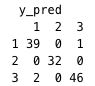
\includegraphics[width=1in]{Figures/svm/svm_cm.png}
    \caption{Support Vector Machine Confusion Matrix}
    \label{fig_svm_cm}
\end{figure}

The final model using the best parameters determined by the \textbf{tune} function is presented in Figure ~\ref{fig_final_svm_model}.

\begin{figure}[H]
    \centering
    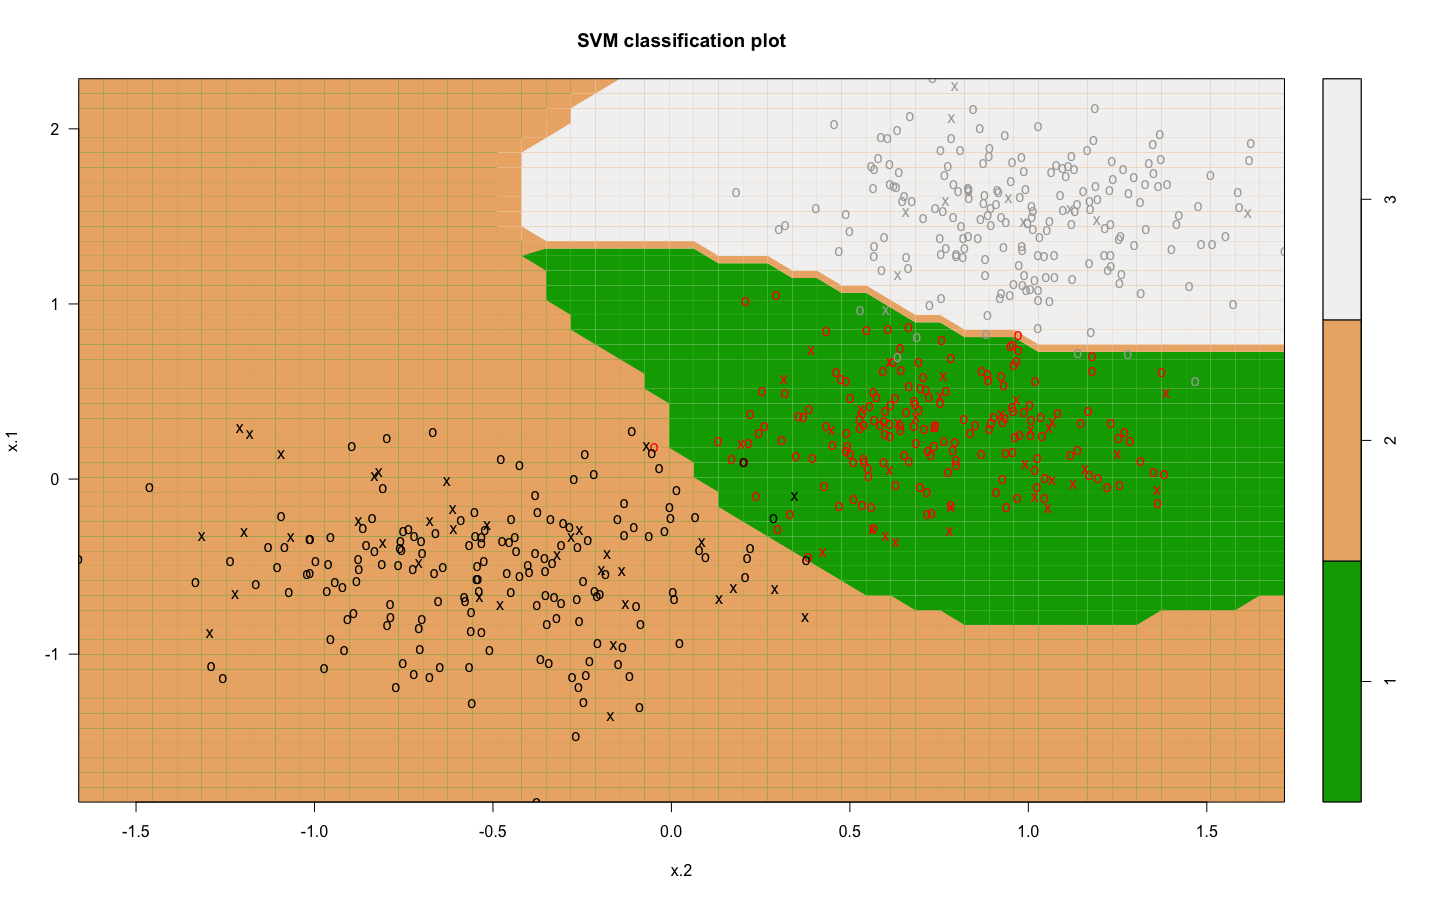
\includegraphics[width=5in]{Figures/svm/svm_final_model.png}
    \caption{Final SVM Model with \(C = 2\) and \(\gamma = 4\)}
    \label{fig_final_svm_model}
\end{figure}

\section{EXAMPLE}

Let us now look at the use of support vector machines in a real dataset. We will be using what is widely known as the Penguin Dataset, collected by Dr. Kristen Gorman and The Palmer Station, Antarctica LTER \cite{penguin_data}. This dataset was originally published in 2014 and includes 7 variables, namely: species, culmen length (mm), culmen depth (mm), flipper length (mm), body mass (g), island, and sex. We transition now into the Python SVM modules from the scikit-learn package to anaylze the Penguin data.

\subsection{DATA EXPLORATION}

We start with importing the necessary modules and functions. The code below sets up our file for later analysis.

\begin{minted}[breaklines]{python3}
    # importing modules
    
    import numpy as np
    from numpy.random import default_rng
    from bokeh.io import output_notebook, show
    from bokeh.plotting import figure
    from bokeh.models import CategoricalColorMapper
    from sklearn.svm import SVC
    rng = default_rng(5)
    output_notebook()
    import pandas as pd

    # importing functions

    def hyperplane(P,x,z=0):
        """Given an SVC object P and an array of vectors x, computes the hyperplane wx+b=z"""
        alphas = P.dual_coef_
        svs = P.support_vectors_
        c = P.intercept_[0]-z
        a = np.sum(alphas.T*svs,axis=0)[0]
        b = np.sum(alphas.T*svs,axis=0)[1]
        return (-c-a*x)/b
\end{minted}

We are now ready to do some initial data exploration. The following code imports the dataset and computes built-in functions associated with dataframes.

\begin{minted}[breaklines]{python3}
    # importing dataset

    df = pd.read_csv('/Users/juliaandronowitz/Desktop/thesis/thesis/ Data/penguins_size.csv')

    # initial exploration of data

    df.head()
    df.info()
    df.isna().sum()
    df.describe()
\end{minted}

The output of these functions is located in Figures ~\ref{fig_df.head()}, ~\ref{fig_df.info()_df.isna().sum()}, and ~\ref{fig_df.describe()}. From Figure ~\ref{fig_df.head()}, we can see the general structure of the dataset. This includes column names and formatting. In Figure ~\ref{fig_df.info()_df.isna().sum()}, the \textbf{df.info()} function tells us the name, length, and type of each variable. We see there are 7 columns and 344 observations. The \textbf{df.isna().sum()} function tells us how many missing values are in each variable. Notice that the variable 'sex' has the most missing observations at a value of 10. Figure ~\ref{fig_df.describe()} describes the basic statistics for the numerical predictors. We see that the data looks clean with no outliers.

\begin{figure}[H]
    \centering
    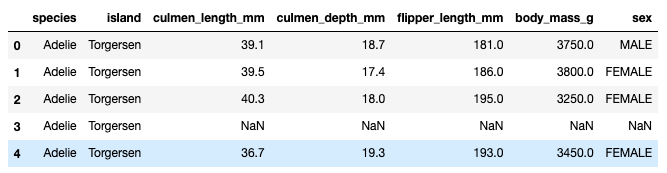
\includegraphics[width=5in]{Figures/penguins/df.head().png}
    \caption{Output of df.head() Function}
    \label{fig_df.head()}
\end{figure}

\begin{figure}[H]
    \centering
    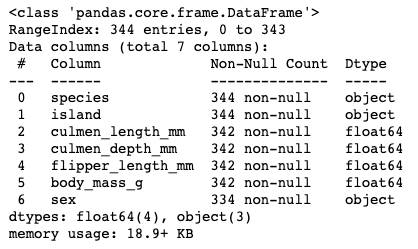
\includegraphics[width=3in]{Figures/penguins/df.info().png}
    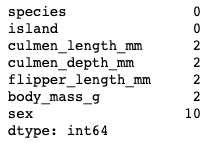
\includegraphics[width=2in]{Figures/penguins/df.isna().sum().png}
    \caption{Output of df.info() and df.isna().sum() Functions}
    \label{fig_df.info()_df.isna().sum()}
\end{figure}

\begin{figure}[H]
    \centering
    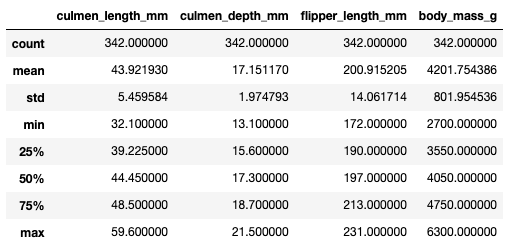
\includegraphics[width=5in]{Figures/penguins/df.describe().png}
    \caption{Output of df.describe() Function}
    \label{fig_df.describe()}
\end{figure}

We now create a function that will tell us the unique values for each variable. This function returns the shape and description of the dataframe that computes the unique values of the predictor. The code is below.

\begin{minted}[breaklines]{python3}
    # a user-defined function to view unique values

    def rstr(df): return df.shape, df.apply(lambda x: [x.unique()])
    rstr(df)
\end{minted}

\begin{figure}[H]
    \centering
    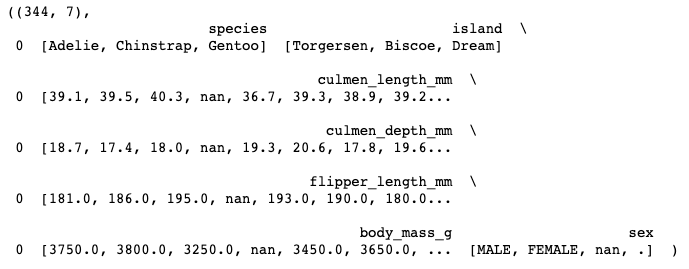
\includegraphics[width=5in]{Figures/penguins/rstr(df).png}
    \caption{Output of rstr(df) Function}
    \label{fig_rstr(df)}
\end{figure}

The unique values in Figure ~\ref{fig_rstr(df)} are useful in determining the species names for the penguins. We see they are Adelie, Chinstrap, and Gentoo. These are important as they are used for the class labels and are what the support vector machine will be trying to predict.

\subsection{CLEANING THE DATA}

From our initial exploration, we notice there are some missing values in the dataset. We first want to drop the missing values. This can be acheived with

\begin{minted}[breaklines]{python3}
    df = df.dropna()
\end{minted}

Next, we are going to need labels for each of our penguin species. These labels will be used when we graph the functions. We also want to color these labels accordingly. Red will be Adelie, blue is Chinstrap, and green is Gentoo.

\begin{minted}[breaklines]{python3}
    labels = []
    x = 0
    for i in df['species']:
        if i == 'Adelie':
            x = 0
        elif i == 'Chinstrap':
            x = 1
        elif i == 'Gentoo':
            x = 2
        labels.append(x)
    
    colors = ['red','blue','green']
    penguin_colors = np.array([colors[i] for i in labels])
\end{minted}

We then want to create a \textbf{numpy} array of the desired variables which will work with the SVM module. We will be removing the species (the class label), island, and sex predictors. This will be the dataset we use in the support vector machine and is located in Figure ~\ref{fig_penguins_numpy}.

\begin{minted}[breaklines]{python3}
    data = df.drop(columns=['species','island','sex'])
    data = data.to_numpy()
\end{minted}

\begin{figure}[H]
    \centering
    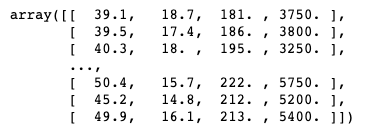
\includegraphics[width=3in]{Figures/penguins/penguins_numpy_data.png}
    \caption{Numpy Array of Penguins Data}
    \label{fig_penguins_numpy}
\end{figure}

\subsection{DATA ANALYSIS}

Now that we have explored and cleaned the data, we can begin analysis. We start by plotting the raw data points for each set of variables. This will help us determine which predictors will be the most useful in the support vector machine.

Below is the code for plotting culmen length and culmen depth. The graph is located in Figure ~\ref{fig_cl_cd}. Recall that the red points correspond to Adelie penguins, blue to Chinstrap, and green to Gentoo. We see that Adelie penguins have a lower culmen length on average than the other species. The Chinstrap penguins have a higher culmen length than the Adelie, but about the same culmen depth. The Gentoo penguins have a lower culmen depth than both the Adelie and Chinstrap. These species have some overlap, but are mostly well-defined. Culmen length and culmen depth may be sufficient predictors for penguin species.

\begin{minted}[breaklines]{python3}
    # plot of culmen length and culmen depth
    cl_cd=figure(title='Penguin Data: culmen length vs. culmen depth')
    cl_cd.scatter(x=data[:,0],y=data[:,1],color=penguin_colors)
    show(cl_cd)
\end{minted}

\begin{figure}[H]
    \centering
    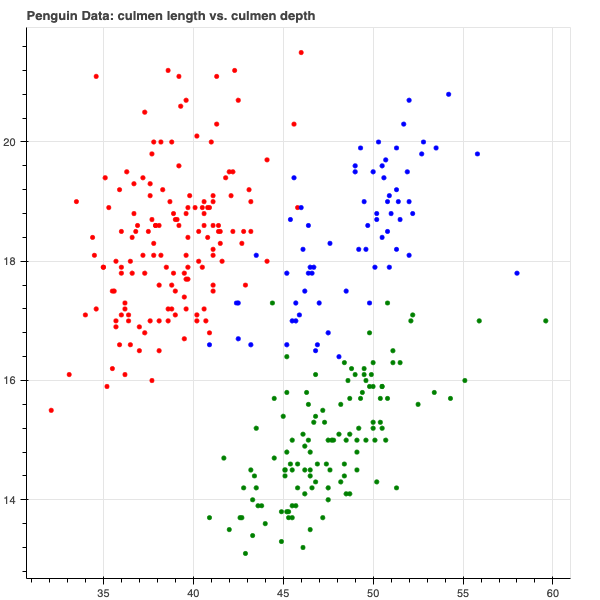
\includegraphics[width=4in]{Figures/penguins/cl_cd.png}
    \caption{Culmen Length vs. Culmen Depth}
    \label{fig_cl_cd}
\end{figure}

Below is the code for plotting culmen length and flipper length. The graph is located in Figure ~\ref{fig_cl_fl}. We see that the Adelie penguins in red have the smallest culmen length and flipper length. Chinstrap penguins have a greater culmen length, while Gentoo penguins have a larger flipper length than the others. Since the three species are pretty well-distinguished, we should look at how these predictors perform in a support vector machine.

\begin{minted}[breaklines]{python3}
    # plot of culmen length and flipper length
    cl_fl=figure(title='Penguin Data: culmen length vs. flipper length')
    cl_fl.scatter(x=data[:,0],y=data[:,2],color=penguin_colors)
    show(cl_fl)
\end{minted}

\begin{figure}[H]
    \centering
    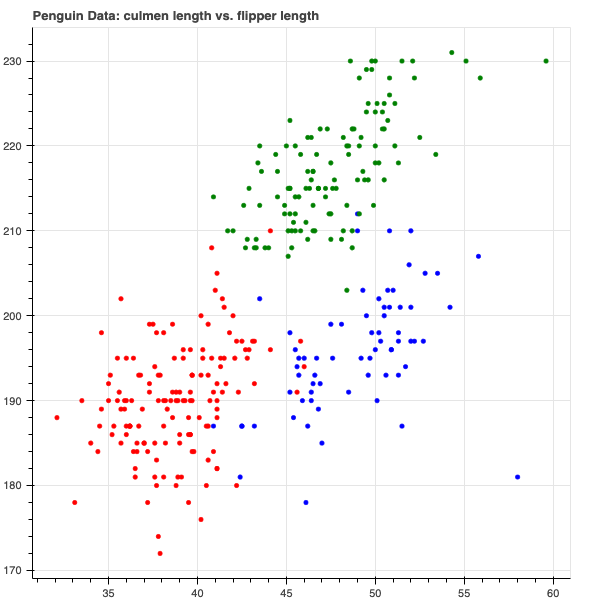
\includegraphics[width=4in]{Figures/penguins/cl_fl.png}
    \caption{Culmen Length vs. Flipper Length}
    \label{fig_cl_fl}
\end{figure}

Next we look at the culmen length and the body mass. The code is located below and the graph in Figure ~\ref{fig_cl_bm}. In this plot, we see a distinction between the three species with some overlap in the Adelie and Gentoo species. The Chinstrap penguins are more set apart with a higher culmen length and lower body mass than the other species. Like the first two graphs, we should see how these variables perform in the classification.

\begin{minted}[breaklines]{python3}
    # plot of culmen length and body mass
    cl_bm=figure(title='Penguin Data: culmen length vs. body mass')
    cl_bm.scatter(x=data[:,0],y=data[:,3],color=penguin_colors)
    show(cl_bm)
\end{minted}

\begin{figure}[H]
    \centering
    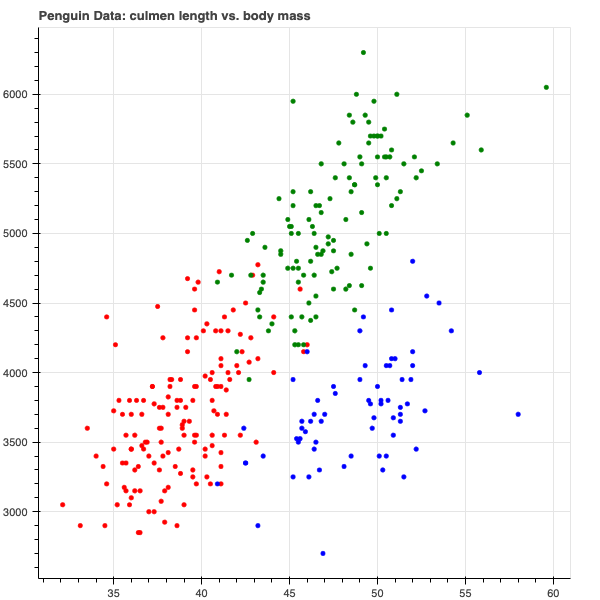
\includegraphics[width=4in]{Figures/penguins/cl_bm.png}
    \caption{Culmen Length vs. Body Mass}
    \label{fig_cl_bm}
\end{figure}

Below is the code for plotting culmen depth and flipper length. The graph is located in Figure ~\ref{fig_cd_fl}. We see there is a clear distinction between the Gentoo penguins and the other two species. However, there is much overlap between the Adelie and Chinstrap penguins. In fact if we didn't have the associated color labels, we would not be able to tell there are supposed to be two groups of penguins represented in that cluster! If we were specifically looking at Gentoo penguins vs. other species, this would be a good choice as there is a clear separating hyperplane. However, culmen depth and flipper length would not be good choices for determing the species of all three penguins. If we were to run a support vector machine with these predictors, we would get many misclassified points and hence a low accuracy.

\begin{minted}[breaklines]{python3}
    # plot of culmen depth and flipper length
    cd_fl=figure(title='Penguin Data: culmen depth vs. flipper length')
    cd_fl.scatter(x=data[:,1],y=data[:,2],color=penguin_colors)
    show(cd_fl)
\end{minted}

\begin{figure}[H]
    \centering
    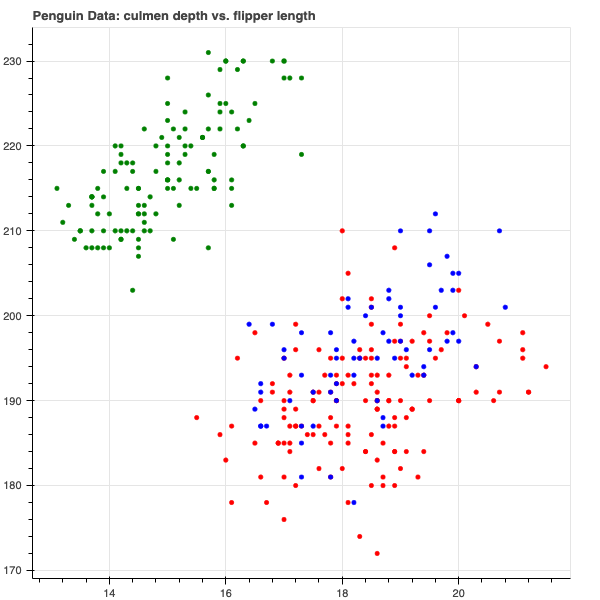
\includegraphics[width=4in]{Figures/penguins/cd_fl.png}
    \caption{Culmen Depth vs. Flipper Length}
    \label{fig_cd_fl}
\end{figure}

Next, we code for the graph of culmen depth and body mass, located in Figure ~\ref{fig_cd_bm}. Much like the culmen depth and flipper length, there is an obvious separation between the Gentoo species and the other two, with Gentoo penguins having a lower culmen depth and higher body mass. These variables would not be a good choice for a multi-class support vector machine.

\begin{minted}[breaklines]{python3}
    # plot of culmen depth and body mass
    cd_bm=figure(title='Penguin Data: culmen depth vs. body mass')
    cd_bm.scatter(x=data[:,1],y=data[:,3],color=penguin_colors)
    show(cd_bm)
\end{minted}

\begin{figure}[H]
    \centering
    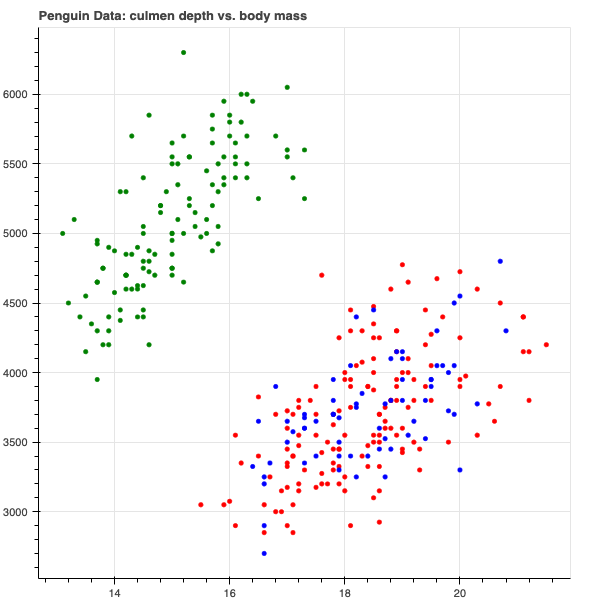
\includegraphics[width=4in]{Figures/penguins/cd_bm.png}
    \caption{Culmen Depth vs. Body Mass}
    \label{fig_cd_bm}
\end{figure}

The last pair of variables to plot is the graph of flipper length and body mass. The graph is located in Figure ~\ref{fig_fl_bm}. We see the Gentoo penguins have different body measurements than the other two species, with Gentoo penguins towards the top right of the graph. The Gentoo species have a higher flipper length and body mass. However, Adelie and Chinstrap penguins have similar flipper length and body mass measurements. These variables would not be a good choice for a support vector machine.

\begin{minted}[breaklines]{python3}
    # plot of culmen depth and body mass
    fl_bm=figure(title='Penguin Data: flipper length vs. body mass')
    fl_bm.scatter(x=data[:,2],y=data[:,3],color=penguin_colors)
    show(fl_bm)
\end{minted}

\begin{figure}[H]
    \centering
    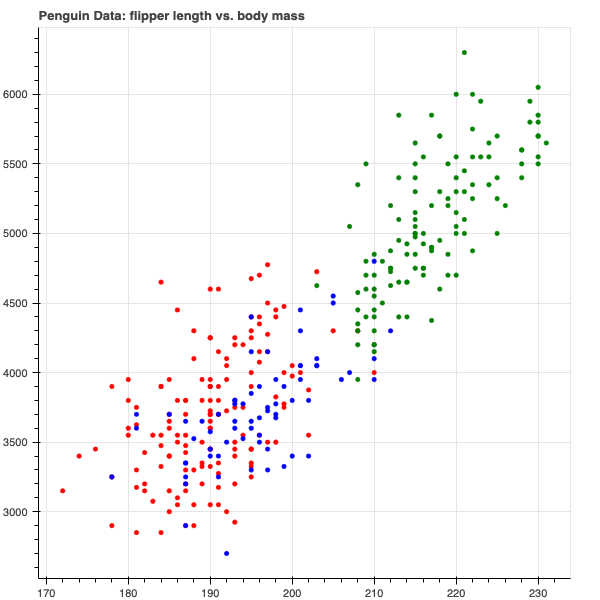
\includegraphics[width=4in]{Figures/penguins/fl_bm.png}
    \caption{Flipper Length vs. Body Mass}
    \label{fig_fl_bm}
\end{figure}

We see the first three plots look the best in separating the three species. The last three graphs have some overlap between the red and blue points, or Adelie and Chinstrap, with the green points, the Gentoo, more clearly distinguishable from the others. Thus, we will perform four different classifications to see which performs the best. Three will be using the variables associated with the first three graphs - culmen length vs. culmen depth, culmen length vs. flipper length, and culmen length vs. body mass - and the last will be a classifier with all four predictors.

\subsection{CULMEN LENGTH VS. CULMEN DEPTH}

We first begin by selecting the necessary columns. The culmen length and culmen depth correspond to the first and second columns in the dataframe. We then need to split our data into training and test datasets. The \textbf{random state} allows the data to be reproducible, much like that of the \textbf{set.seed()} function in \textit{R}.

\begin{minted}[breaklines]{python3}
    # selecting columns
    data_cl_cd = data[:,[0,1]]

    # splitting into training and test data
    x_train, x_test, y_train, y_test = train_test_split(data_cl_cd, labels, test_size = 0.20, random_state=30)
\end{minted}

We then fit our model to specified cost and gamma values. We use the training sets to create the model, then use the model to predict the species based on the culmen depth and culmen length in the test set. We then print the accuracy of the model when used on the test set.

\begin{minted}[breaklines]{python3}
    fit_cl_cd = SVC(kernel = 'rbf', C=1, gamma=1).fit(x_train,y_train)
    fit_cl_cd.predict(x_test)
    print('Classifier yields accuracy of {:2f}%'.format(fit_cl_cd.score(x_test,y_test)))   
\end{minted}

This gives us an output of 95.5\(\%\). Could we achieve a higher accuracy? The \textbf{GridSearch} function gives us a method to calculate the accuracies of many different cost and gamma combinations \cite{svm_python_tuning}. The code below sets a list of cost and gamma values that the function fits to the training data. We can see the best parameters using the \textbf{best estimator} line.

\begin{minted}[breaklines]{python3}
    param_grid = {'C': [0.01, 0.1,1, 10, 100, 1000], 'gamma': [1,0.1,0.01,0.001,'auto','scale'],'kernel': ['rbf']}
    grid = GridSearchCV(fit_cl_cd,param_grid,refit=True,verbose=2)
    grid.fit(x_train,y_train)

    # best parameters
    print(grid.best_estimator_)
\end{minted}

We can now see that the model fit to these parameters yields an accuracy of 97.0\%.

\begin{minted}[breaklines]{python3}
    fit_cl_cd = SVC(kernel = 'rbf', C=1000, gamma=0.01).fit(x_train,y_train)
    fit_cl_cd.predict(x_test)
    print('Classifier yields accuracy of {:2f}%'.format(fit_cl_cd.score(x_test,y_test)))
\end{minted}

Using this model, we can create a graph of the support vector machine's decision boundary, as described in \cite{scikit_svm_plotting}.

\begin{minted}[breaklines]{python3}
    fig, ax = plt.subplots()

    h = .02
    
    # create a mesh to plot in
    x_min, x_max = data[:, 0].min() - 1, data[:, 0].max() + 1
    y_min, y_max = data[:, 1].min() - 1, data[:, 1].max() + 1
    xx, yy = np.meshgrid(np.arange(x_min, x_max, h),
                         np.arange(y_min, y_max, h))
    
    Z = fit_cl_cd.predict(np.c_[xx.ravel(), yy.ravel()])
    
    # put the result into a color plot
    Z = Z.reshape(xx.shape)
    ax.contourf(xx, yy, Z, cmap=plt.cm.coolwarm, alpha=0.8)
    
    # create the scatterplot
    scatter = ax.scatter(data[:, 0], data[:, 1], c=labels, cmap=plt.cm.coolwarm, edgecolors='black')
    
    # produce a legend with the unique colors from the scatter
    legend1 = ax.legend(*scatter.legend_elements(), bbox_to_anchor=(1, 0.5), title="Classes")
    ax.add_artist(legend1)
    
    # add axis labels
    ax.set_xlabel("Culmen Length")
    ax.set_ylabel("Culmen Depth")
    
    plt.show()    
\end{minted}

The output of the code is shown in Figure ~\ref{fig_fit_cl_cd}. Our first support vector machine has the potential for accurately determining a penguin's species based on the culmen length and culmen depth predictors.

\begin{figure}[H]
    \centering
    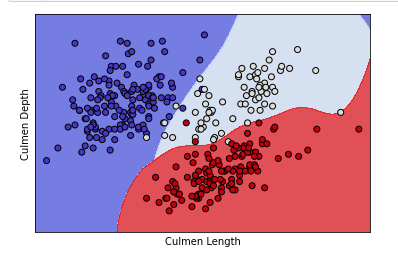
\includegraphics[width=5in]{Figures/penguins/fit_cl_cd.png}
    \caption{Final SVM Module of Culmen Length vs. Culmen Depth}
    \label{fig_fit_cl_cd}
\end{figure}

\subsection{CULMEN LENGTH VS. FLIPPER LENGTH}

We now repeat the process for the culmen length and flipper length variables, selecting the required columns and splitting into training and test data.

\begin{minted}[breaklines]{python3}
    # selecting columns
    data_cl_fl = data[:,[0,2]]

    # splitting into training and test data
    x_train, x_test, y_train, y_test = train_test_split(data_cl_fl, labels, test_size = 0.20, random_state=30)
\end{minted}

We now fit our model to specified cost and gamma values and print the accuracy of the model when used on the test set.

\begin{minted}[breaklines]{python3}
    fit_cl_fl = SVC(kernel = 'rbf', C=1, gamma=1).fit(x_train, y_train)
    fit_cl_fl.predict(x_test)
    print('Classifier yields accuracy of {:2f}%'.format(fit_cl_fl.score(x_test,y_test)))  
\end{minted}

This has an accuracy of 88.1\%. We again use the \textbf{GridSearch} function to determine the best parameters.

\begin{minted}[breaklines]{python3}
    # using the GridSearch function
    param_grid = {'C': [0.01, 0.1,1, 10, 100, 1000], 'gamma': [1,0.1,0.01,0.001,'auto','scale'],'kernel': ['rbf']}
    grid = GridSearchCV(fit_cl_fl,param_grid,refit=True,verbose=2)
    grid.fit(x_train,y_train)
    print(grid.best_estimator_)
    
    # fitting the model
    fit_cl_fl = SVC(kernel = 'rbf', C=10, gamma=0.01).fit(x_train,y_train)
    fit_cl_fl.predict(x_test)
    print('Classifier yields accuracy of {:2f}%'.format(fit_cl_fl.score(x_test,y_test)))
\end{minted}

We can now see that the model fit to these parameters yields an accuracy of 97.0\%, which is much higher. Using this model, we can create a graph of the support vector machine's decision boundary.

\begin{minted}[breaklines]{python3}
    fig, ax = plt.subplots()

    h = .02
    
    # create a mesh to plot in
    x_min, x_max = data[:, 0].min() - 1, data[:, 0].max() + 1
    y_min, y_max = data[:, 2].min() - 1, data[:, 2].max() + 1
    xx, yy = np.meshgrid(np.arange(x_min, x_max, h),
                         np.arange(y_min, y_max, h))
    
    Z = fit_cl_fl.predict(np.c_[xx.ravel(), yy.ravel()])
    
    # Put the result into a color plot
    Z = Z.reshape(xx.shape)
    ax.contourf(xx, yy, Z, cmap=plt.cm.coolwarm, alpha=0.8)
    
    scatter = ax.scatter(data[:, 0], data[:, 2], c=labels, cmap=plt.cm.coolwarm, edgecolors='black')
    
    # produce a legend with the unique colors from the scatter
    legend1 = ax.legend(*scatter.legend_elements(), bbox_to_anchor=(1, 0.5), title="Classes")
    ax.add_artist(legend1)
    
    # add axis labels
    ax.set_xlabel("Culmen Length")
    ax.set_ylabel("Flipper Length")
    
    plt.show()      
\end{minted}

The output of the code is shown in Figure ~\ref{fig_fit_cl_fl}. Adelie penguins have a class label of 0 with Chinstrap and Gentoo being 1 and 2, respectively. Overall, this seems like a good choice of predictors for a support vector machine that predicts a penguin's species.

\begin{figure}[H]
    \centering
    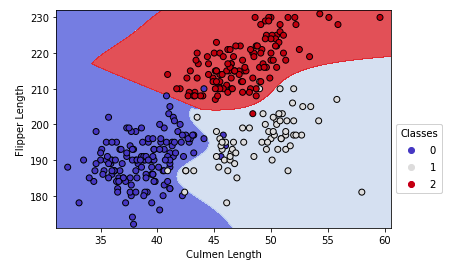
\includegraphics[width=5in]{Figures/penguins/fit_cl_fl.png}
    \caption{Final SVM Module of Culmen Length vs. Flipper Length}
    \label{fig_fit_cl_fl}
\end{figure}

\subsection{CULMEN LENGTH VS. BODY MASS}

The initial process for the model using culmen length and body mass closely follows that of the previous two.

\begin{minted}[breaklines]{python3}
    # selecting columns
    data_cl_bm = data[:,[0,3]]

    # split into training and test data
    x_train, x_test, y_train, y_test = train_test_split(data_cl_bm, labels, test_size = 0.20, random_state=30)

    # fitting model to specified values
    fit_cl_bm = SVC(kernel = 'rbf', C=1, gamma=1).fit(x_train,y_train)
    fit_cl_bm.predict(x_test)
    print('Classifier yields accuracy of {:2f}%'.format(fit_cl_bm.score(x_test,y_test)))
\end{minted}

The first model we create yields an accuracy of 74.6\%, which is not great! We now try to find better parameters to use.

\begin{minted}[breaklines]{python3}
    # using GridSearch
    param_grid = {'C': [0.01, 0.1,1, 10, 100, 1000], 'gamma': [1,0.1,0.01,0.001,'auto','scale'],'kernel': ['rbf']}
    grid = GridSearchCV(fit_cl_bm,param_grid,refit=True,verbose=2)
    grid.fit(x_train,y_train)

    print(grid.best_estimator_)

    # fitting new model
    fit_cl_bm = SVC(kernel = 'rbf', C=1000, gamma=0.001).fit(x_train,y_train)
    fit_cl_bm.predict(x_test)
    print('Classifier yields accuracy of {:2f}%'.format(fit_cl_bm.score(x_test,y_test)))
\end{minted}

The second model we create has an accuracy of 79.1\%. This is much lower than our other two models. Nevertheless, we try to plot the decision boundary to get a better idea of the support vector machine. When running the code similar to the graphs from the first two, the machine crashes. This presented us with an unusual problem, which we debugged to boil down to the step size. Where the other two models had y-axis that were in the hundreds, a step size $h$ of 0.02 was a good choice. However, the body mass of the penguins is measured in grams which ends up with a mean in the thousands. Thus, a step size of 0.02 with the scale of the y-axis in the third model is not feasible. While we can adjust the step size to a larger value and end up with the plot in Figure ~\ref{fig_fit_cl_bm} which is produced by the code below, it is better to rescale the data.

\begin{minted}[breaklines]{python3}
    fig, ax = plt.subplots()

    h = 1
    
    # create a mesh to plot in
    x_min, x_max = data[:, 0].min() - 1, data[:, 0].max() + 1
    y_min, y_max = data[:, 3].min() - 1, data[:, 3].max() + 1
    xx, yy = np.meshgrid(np.arange(x_min, x_max, h),
                         np.arange(y_min, y_max, h))
    
    Z = fit_cl_bm.predict(np.c_[xx.ravel(), yy.ravel()])
    
    # Put the result into a color plot
    Z = Z.reshape(xx.shape)
    ax.contourf(xx, yy, Z, cmap=plt.cm.coolwarm, alpha=0.8)
    
    scatter = ax.scatter(data[:, 0], data[:, 3], c=labels, cmap=plt.cm.coolwarm, edgecolors='black')
    
    # produce a legend with the unique colors from the scatter
    legend1 = ax.legend(*scatter.legend_elements(), bbox_to_anchor=(1, 0.5), title="Classes")
    ax.add_artist(legend1)
    
    # add axis labels
    ax.set_xlabel("Culmen Length")
    ax.set_ylabel("Body Mass")
    
    plt.show()    
\end{minted}

\begin{figure}[H]
    \centering
    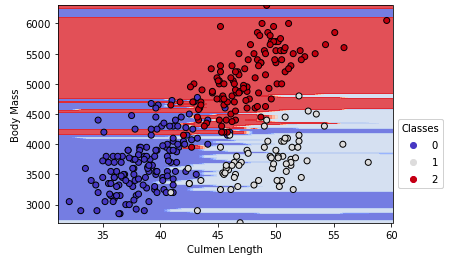
\includegraphics[width=5in]{Figures/penguins/fit_cl_bm.png}
    \caption{Initial SVM Module of Culmen Length vs. Body Mass}
    \label{fig_fit_cl_bm}
\end{figure}

To scale the data, we divide the body mass by 10.

\begin{minted}[breaklines]{python3}
    data_cl_bm[:,[1]]=data_cl_bm[:,[1]]/10
\end{minted}

The steps to produce the classifier are now the same as those above. We see the initial model with a cost and gamma both of 1 yields an accuracy of 74.63\%. Once performing the grid search, we try with the cost parameter of 100 and gamma of 0.001. This yields 91.04\% which is remarkably better than the final model produced by the unscaled data! With a step size of 0.1, we see the class boundaries of the classifier much more clearly in Figure ~\ref{fig_fit_scaled_cl_bm}.

\begin{figure}[H]
    \centering
    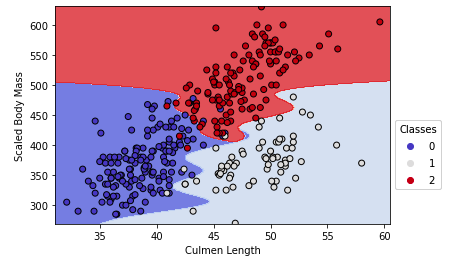
\includegraphics[width=5in]{Figures/penguins/fit_scaled_cl_bm.png}
    \caption{Scaled SVM Module of Culmen Length vs. Body Mass}
    \label{fig_fit_scaled_cl_bm}
\end{figure}

While the classifier using the culmen depth and body mass improved greatly, the best tuned machine using culmen length and body mass has a lower accuracy than our attempts with culmen length and both culmen depth and flipper length.

\subsection{ALL 4 PREDICTORS}

Support vector machines are known to perform well in high-dimensional spaces. We now try a support vector machine using all 4 predictors to investigate whether this model will perform better than those with only two predictors.

\begin{minted}[breaklines]{python3}
    # splitting data
    x_train, x_test, y_train, y_test = train_test_split(data, labels, test_size = 0.20, random_state=30)
    
    # fitting model
    fit_all = SVC(kernel = 'rbf', C=1, gamma=1).fit(x_train,y_train)
    fit_all.predict(x_test)
    print('Classifier yields accuracy of {:2f}%'.format(fit_all.score(x_test,y_test)))
\end{minted}

The first attempt yields an accuracy of 55.2\%! This is by far the least-performing model. Let us see if tuning the model provides significant improvement.

\begin{minted}[breaklines]{python3}
    # tuning
    param_grid = {'C': [0.01, 0.1,1, 10, 100, 1000], 'gamma': [1,0.1,0.01,0.001,'auto','scale'],'kernel': ['rbf']}
    grid = GridSearchCV(fit_all,param_grid,refit=True,verbose=2)
    grid.fit(x_train,y_train)
    print(grid.best_estimator_)

    # final fit
    fit_all = SVC(kernel = 'rbf', C=10, gamma=0.001).fit(x_train,y_train)
    fit_all.predict(x_test)
    print('Classifier yields accuracy of {:2f}%'.format(fit_all.score(x_test,y_test)))
\end{minted}

This machine yields an accuracy of 79.1\%. While this is better than before, it does not outperform either of the first two models. This would not be a good choice for a support vector machine.

\subsection{RESULTS}

We see the support vector machine using the culmen length and culmen depth or the culmen length and flipper length as the predictors had the highest accuracy, both at $97.0\%$. The model with all 4 predictors and the culmen length and body mass as predictors performed the worst, with accuracies of 79.1\%. We should choose either of the first two models when attempting to predict penguin species.

\section{APPLICATIONS}

One such example, as presented in \textit{Intro to Statistical Learning with Applications in R} \citep{introstatlearning} is the use of support vector machines in genetic expression data. The \textit{Khan} dataset in the $ISLR2$ package of $R$ contains expression measurements for 2,308 genes from tissue samples of patients with one of four types of small round blue cell tumors. The data is then split up into training and test groups. There are 63 observations in the training set and 20 observations in the test set. It is not feasible to visually plot the data on a graph, as there is a very large number of features relative to the number of observations. However, due to the large number of features, it is easy to find a linearly separating hyperplane that predicts the type of cell tumor. As such, the SVM approach outlined in the textbook yields no data points that are misclassified in the training set and two test set errors. In this case, a support vector machine was used to classify and predict cancer types based on gene expression data. In fact, SVMs are a popular choice in machine learning approaches to detecting cancer. Several studies have shown SVMs perform with great accuracy. Among those include the prediction of breast cancer using SVM and an extremely randomized trees classifier \cite{breastcancer}. Support vector machines have also been used in multi-class lung cancer classification \cite{lungcancer}.

\section{ANALYSIS OF R AND PYTHON SVM MODULES AND DOCUMENTATION}

We now compare the SVM modules for $R$ and Python. The supporting documentation for the \textit{scikitlearn} module can be found in \cite{scikit_svm} and \textit{e1071} in \cite{e1071}. The $R$ and Python modules for support vector machines are quite similar in terms of the variables calculated. Table ~\ref{tab_r_python} provides a summary of the corresponding variables in each program. The $P$ refers to the model created by the \textbf{svm} function. 

\begin{table}[H]
    \centering
    \def\arraystretch{1.5}
    \begin{tabular}{c|c}
        $R$'s \textit{e1071} & Python's \textit{scikitlearn} \\
        \hline
        -1$*$P\$coefs & P.dual\_coef\_ \\
        data[P\$index,] & P.support\_vectors\_ \\
        P\$rho & P.intercept\_
    \end{tabular}
    \caption{Parameters in $R$ and Python}
    \label{tab_r_python}
\end{table}

The SVM modules in both programming languages are similar. Python's \textit{scikitlearn} and $R$'s \textit{e1071} both use a one-vs-one approach in multi-class models. The mathematical formulation for the Python classifier can be accessed through \cite{scikit_svm}. On the other hand, the $R$ module was based on $C/C++$ code. Thus, the mathematical formulation is said to follow that of Chih-Chung Chang and Chih-Jen Lin in
LIBSVM: a library for Support Vector Machines, found in https://www.csie.ntu.edu.tw/~cjlin/papers/libsvm.ps.gz. This file proved cumbersome to open and is not as accessible as that of \textit{scikitlearn}.

When it comes to plotting, Python offers much more flexible and intuitive tools. While the code can get quite long, the plots are aesthetic and customizable. While there are options for plotting in $R$, it is not as readily available and felt more rigid and elementary.

From my experience, Python's documentation was much easier to find, follow, and consult than $R$'s. While both $R$ and Python have similar mathematical capabilities regarding the \textbf{svm} module, the more accessible documentation as well as the superior graphics and adjustability of the language make Python the preferable choice in future analyses.

\section{Conclusion}
In this paper, we first discussed the evolution of machine learning and artificial intelligence where types of supervised and unsupervised learning were covered. Then came the concept of hyperplanes, in which we established the mathematical formulas in various dimensions with visualizations. This was crucial in the discussion of the maximal margin classifier, where linearly separable groups were classified using a hyperplane. Non-linearly separable groups were the focus of the support vector classifier, in which the cost played a large part in determining the number of support vectors. The gamma variable was introduced in the support vector machine, as it provided a measure of 'curviness' in the use of kernels with non-linear data. Finally, a support vector machine was used to classify penguin species based on certain predictors. Various models were calculated, validated, and graphed in this real dataset. The documentation for the $R$ and Python \textbf{svm} modules were compared as a means to determine the differences between each when going forth with further projects. Overall, this paper gave an introduction to the concept of support vector machines and the various associated classification methods.

\newpage
\thispagestyle{empty}

\bibliography{References/References.bib}

\end{document}
